	\begin{frame}{Huấn luyện mạng nơ-ron đa lớp - Bộ dữ liệu thực nghiệm}
	   \begin{table}
        \centering
    	\begin{tabular}{|c|c|c|c|c|}
            \hline
            {\textbf{STT}} & 
            \multicolumn{1}{c|} {\textbf{Bài toán}} & \multicolumn{1}{c|}{\textbf{Số đơn vị đầu vào}} &  \multicolumn{1}{c|}{\textbf{Tổng số điểm dữ liệu}}\\ \hline
            1 & 4-bit & 4  & 16 \\\hline
            2 & 6-bit & 6  & 64 \\\hline
            3 & 8-bit & 8  & 256 \\\hline
            4 & 9-bit & 9  & 512 \\\hline
            5 & 10-bit & 10  & 1024 \\\hline
            6 & Breast cancer & 9  & 699 \\\hline
            7 & Tic-tac-toe & 9  & 958 \\\hline
            8 & Ionosphere & 34  & 351 \\\hline
            9 & Credit screening & 14  & 653 \\\hline
        \end{tabular}
        \label{tab:result:nbit}
        \caption{Các bài toán phân loại nhị phân dùng trong thực nghiệm}
    \end{table}
	\end{frame}
	\begin{frame}{Thực nghiệm}
	    \begin{table}[h!]
        	\begin{tabular}{|l|c|c|}
                \hline
                \multirow{1}{*}{\textbf{Tham số}} & 
                \multicolumn{1}{c|} {\textbf{Ký hiệu}} & \multicolumn{1}{c|}{\textbf{Giá trị}}\\ \hline
                Kích thước quần thể đơn nhiệm &  & 30\\
                Kích thước quần thể đa nhiệm &  & 30\\
                Số thế hệ tiến hóa &  & 1000\\
                Chỉ số phân phối SBX &  & 15\\
                Tỉ lệ đột biến PMU &  & 0.2\\
                Chỉ số đột biến PMU &  & 15\\
                pswap & & 0.5\\
                Giá trị tham số cố định $rmp$ của thuật toán $MFEA$ &  & 0.5\\
                Giá trị khởi tạo các phần tử trong ma trận $RMP$ &  & 0\\
                Giá trị chặn dưới của từng phần tử $rmp_{kj}, k,j \in {K}$  &  & 0.1\\
                Số lần chạy thống kê & & 30\\ \hline
                
        
            \end{tabular}
            \label{tab:config:nbit}
            \caption{Cấu hình và tham số giải thuật đề xuất cho bài toán huấn luyện các mạng nơ-ron đa lớp}
        \end{table}
	\end{frame}
	\begin{frame}{Cấu hình tác vụ}
	    \begin{table}[h!]
        \centering
    	\begin{tabular}{|c|c|c|c|c|}
            \hline
            \multirow{1}{*}{\textbf{Bài toán}} & 
            \multicolumn{1}{c|} {\textbf{Tên tác vụ}} & \multicolumn{1}{c|}{\textbf{Cấu trúc lần lượt của từng tác vụ}}\\ \hline
            
            \multirow{1}{*}
            {4bit} 
            &  4bit (4-5-6) &  (4,4,1)-(4,5,1)-(4,6,1)\\\hline
            \multirow{2}{*} 
            {6bit} 
            &  6bit (5-6-7) & (6,5,1)-(6,6,1)-(6,7,1)\\ \cline{2-3}
            &  6bit (6-7-8) & (6,6,1)-(6,7,1)-(6,8,1)\\ \hline
            \multirow{2}{*} 
            {8bit} 
            &  8bit (5-6-7) & (8,5,1)-(8,6,1)-(8,7,1)\\\cline{2-3}
            &  8bit (6-7-8) & (8,6,1)-(8,7,1)-(8,8,1)\\\hline

        \end{tabular}
        \label{tab:result:nbit}
        \caption{Bài toán huấn luyện mạng nơ-ron 1 lớp ẩn đơn giản}
    \end{table}
    \begin{table}[h!]
        \centering
    	\begin{tabular}{|c|c|c|c|c|}
            \hline
            \multirow{2}{*}{\textbf{Bài toán}} & 
            \multicolumn{2}{c|} {\textbf{ANN cùng độ sâu}} & \multicolumn{2}{c|}{\textbf{ANN khác độ sâu}}\\ \cline{2-5}
            &\multicolumn{1}{c|} {\textbf{Tên tác vụ}} & \multicolumn{1}{c|}{\textbf{Cấu trúc mạng}} & \multicolumn{1}{c|} {\textbf{Tên tác vụ}} & \multicolumn{1}{c|}{\textbf{Cấu trúc mạng}}\\ \hline
            
            \multirow{3}{*} 
            {8bit} &  Tác vụ 1 & (6,2) & Tác vụ 1 & (2,2,2,2,2) \\ \cline{2-5}
             & Tác vụ 2 & (6,3) & Tác vụ 2 & (2,2,2,2)\\ \cline{2-5}
            & Tác vụ 3 & (6,4) & Tác vụ 3 & (2,2,2)\\ \hline
            \multirow{3}{*} 
            {9bit} &  Tác vụ 1 & (6,2) & Tác vụ 1 & (2,2,2,2,2) \\ \cline{2-5}
             & Tác vụ 2 & (6,3) & Tác vụ 2 & (2,2,2,2)\\ \cline{2-5}
            & Tác vụ 3 & (6,4) & Tác vụ 3 & (2,2,2) \\ \hline
            \multirow{3}{*} 
            {10bit} &  Tác vụ 1 & (6,2) & Tác vụ 1 & (2,2,2,2,2) \\ \cline{2-5}
             & Tác vụ 2 & (6,3) & Tác vụ 2 & (2,2,2,2)\\ \cline{2-5}
            & Tác vụ 3 & (6,4) & Tác vụ 3 & (2,2,2)\\ \hline
        \end{tabular}
        \label{tab:result:nbit}
        \caption{Bộ dữ liệu huấn luyện nhiều mô mạng Nơ-ron đa lớp}
    \end{table}
	\end{frame}
	
	\begin{frame}{Cấu hình tác vụ}
    \begin{table}[h!]
        \centering
    	\begin{tabular}{|c|c|c|c|c|}
            \hline
            \multirow{2}{*}{\textbf{Bài toán}} & 
            \multicolumn{2}{c|} {\textbf{ANN cùng độ sâu}} & \multicolumn{2}{c|}{\textbf{ANN khác độ sâu}}\\ \cline{2-5}
            &\multicolumn{1}{c|} {\textbf{Tên tác vụ}} & \multicolumn{1}{c|}{\textbf{Cấu trúc mạng}} & \multicolumn{1}{c|} {\textbf{Tên tác vụ}} & \multicolumn{1}{c|}{\textbf{Cấu trúc mạng}}\\ \hline
            
            \multirow{3}{*} 
            {ionosphere} &  Tác vụ 1 & (5,2) & Tác vụ 1 & (2,2,2,2,2) \\ \cline{2-5}
             & Tác vụ 2 & (5,3) & Tác vụ 2 & (2,2,2,2)\\ \cline{2-5}
            & Tác vụ 3 & (5,4) & Tác vụ 3 & (2,2,2)\\ \hline
            \multirow{3}{*} 
            {ticTacToe} &  Tác vụ 1 & (5,2) & Tác vụ 1 & (2,2,2,2,2) \\ \cline{2-5}
             & Tác vụ 2 & (5,3) & Tác vụ 2 & (2,2,2,2)\\ \cline{2-5}
            & Tác vụ 3 & (5,4) & Tác vụ 3 & (2,2,2) \\ \hline
            \multirow{3}{*} 
            {creditScreening} &  Tác vụ 1 & (6,2) & Tác vụ 1 & (2,2,2,2,2) \\ \cline{2-5}
             & Tác vụ 2 & (6,3) & Tác vụ 2 & (2,2,2,2)\\ \cline{2-5}
            & Tác vụ 3 & (6,4) & Tác vụ 3 & (2,2,2)\\ \hline
            \multirow{3}{*} 
            {breastCancer} &  Tác vụ 1 & (6,2) & Tác vụ 1 & (2,2,2,2,2) \\ \cline{2-5}
             & Tác vụ 2 & (6,3) & Tác vụ 2 & (2,2,2,2)\\ \cline{2-5}
            & Tác vụ 3 & (6,4) & Tác vụ 3 & (2,2,2)\\ \hline
        \end{tabular}
        \label{tab:result:nbit}
        \caption{Bộ dữ liệu huấn luyện UCI}
    \end{table}
	\end{frame}
	\begin{frame}{6-bit even problem}
		\begin{table} [H]
        	\caption{Bài 4 bit 1 lớp ẩn}
            \begin{center}
            \begin{tabular}{|c|c|c|c|}
            \hline
            \multirow{1}{*}{\textbf{Method}} & \multicolumn{1}{c|}{\textbf{Subtask1}} & \multicolumn{1}{c|}{\textbf{Subtask 2}} & \multicolumn{1}{c|}{\textbf{Subtask 3}} \\ \hline
            CEA & $0.0316 \pm 0.0125$ & $0.0201 \pm 0.011922$ & $0.0117 \pm 0.008133$ \\
            MFEA-I & $0.025 \pm 0.012957$ & $0.0117 \pm 0.007342$ & $0.0072 \pm 0.005355$\\
            MFEA-II  & $\mathbf{0.0219 \pm 0.009181}$ & $\mathbf{0.0099 \pm 0.007053}$ & $\mathbf{0.0052 \pm 0.004126}$ \\\hline
            
            \end{tabular}
            \end{center}
            
            \label{tab:result:nbit}
            \caption{6-bit even parity problem}
            \begin{center}
            \begin{tabular}{|c|c|c|c|}
            \hline
            \multirow{1}{*}{\textbf{Method}} & \multicolumn{1}{c|}{\textbf{Subtask1}} & \multicolumn{1}{c|}{\textbf{Subtask 2}} & \multicolumn{1}{c|}{\textbf{Subtask 3}} \\ \hline
            CEA(5,6,7)  & $0.0703 \pm 0.014543$ & $0.0619 \pm 0.018078$ & $0.0572 \pm 0.017982$ \\
            MFEA-I(5,6,7)   & $\mathbf{0.06 \pm 0.014702}$ & $\mathbf{0.0498 \pm 0.009562}$ & $0.047 \pm 0.008464$ \\
            MFEA-II(5,6,7)  & $0.06 \pm 0.011387$ & $0.052 \pm 0.009393$ & $\mathbf{0.047 \pm 0.009579}$ \\\hline
            
            CEA(6,7,8)   & $0.0669 \pm 0.016032$ & $0.0583 \pm 0.009948$ & $0.0521 \pm 0.015598$ \\
            MFEA-I(6,7,8)  & $0.0611 \pm 0.013622$ & $0.0528 \pm 0.011122$ & $0.0484 \pm 0.011074$ \\
            MFEA-II(6,7,8) & $\mathbf{0.0522 \pm 0.011066}$ & $\mathbf{0.0476 \pm 0.01033}$ & $\mathbf{0.0418 \pm 0.011741}$ \\\hline
            
            \end{tabular}
            \end{center}
        \end{table}
	\end{frame}
	
    \begin{frame}{8-bit even problem}
    \begin{table} [H]
        \caption{8-bit even parity problem}
        \begin{center}
        \begin{tabular}{|c|c|c|c|}
        \hline
        \multirow{1}{*}{\textbf{Method}} & \multicolumn{1}{c|}{\textbf{Subtask1}} & \multicolumn{1}{c|}{\textbf{Subtask 2}} & \multicolumn{1}{c|}{\textbf{Subtask 3}} \\ \hline
        CEA(5,6,7) & $0.0956 \pm 0.013764$ & $0.0906 \pm 0.015274$ & $0.0874 \pm 0.010884$ \\
        MFEA-I(5,6,7) & $0.0859 \pm 0.011722$ & $0.0801 \pm 0.009489$ & $0.0778 \pm 0.010507$  \\
        MFEA-II(5,6,7) & $\mathbf{0.0827 \pm 0.010678}$ & $\mathbf{0.076 \pm 0.012979}$ & $\mathbf{0.0735 \pm 0.012598}$ \\\hline
        
        CEA(6,7,8)& $0.0895 \pm 0.012499$ & $0.0902 \pm 0.013171$ & $0.081 \pm 0.013371$ \\
        MFEA-I(6,7,8)  & $0.0826 \pm 0.011089$ & $0.0768 \pm 0.010228$ & $0.0734 \pm 0.008805$ \\
        MFEA-II(6,7,8) & $\mathbf{0.0808 \pm 0.010726}$ & $\mathbf{0.0739 \pm 0.01117}$ & $\mathbf{0.072 \pm 0.009657}$ \\\hline
        \end{tabular}
        \end{center}
        
        \label{tab:result:nbit}
    \end{table}
    \end{frame}
    \begin{frame}{Bài 4bit}
        \begin{figure}[H]
            \centering
            \scalebox{.6}{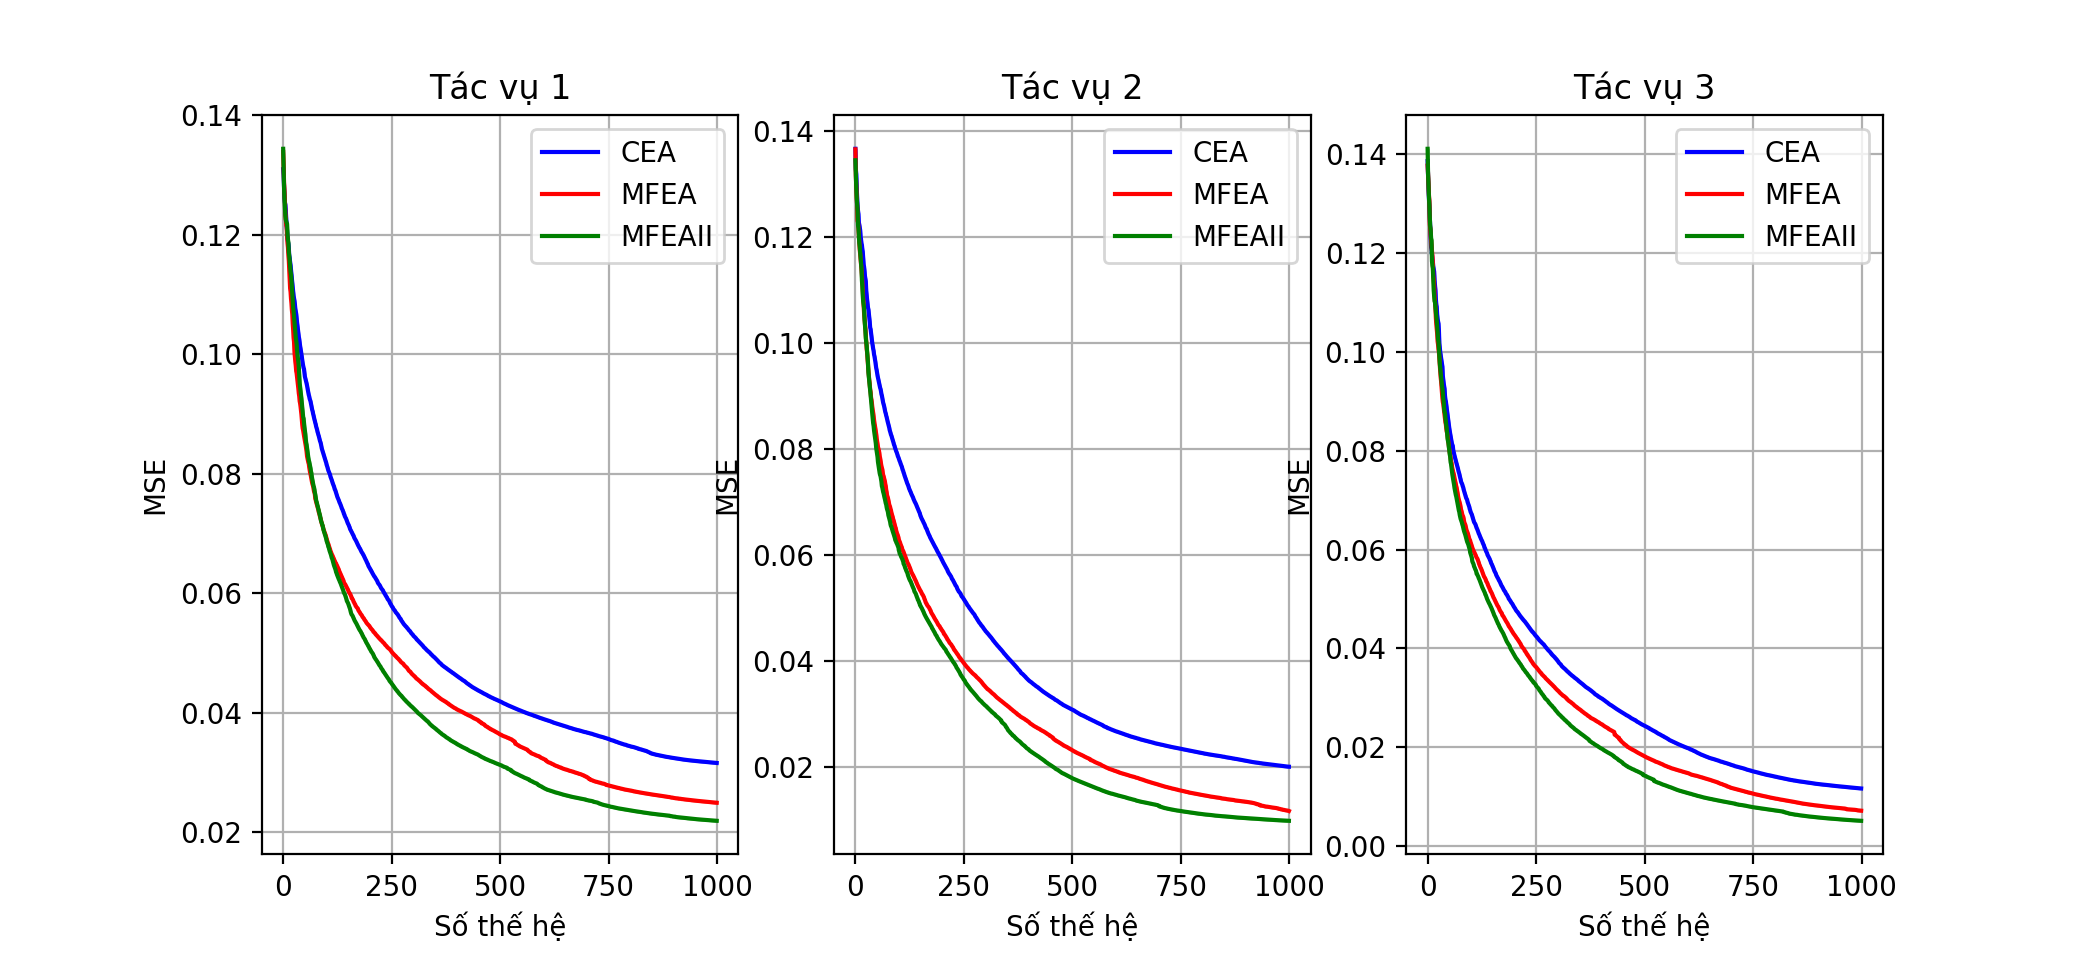
\includegraphics[width=\textwidth,height=\textheight,keepaspectratio]{images/results/nbit_1layer/4bit_task.png}}
            \scalebox{.6}{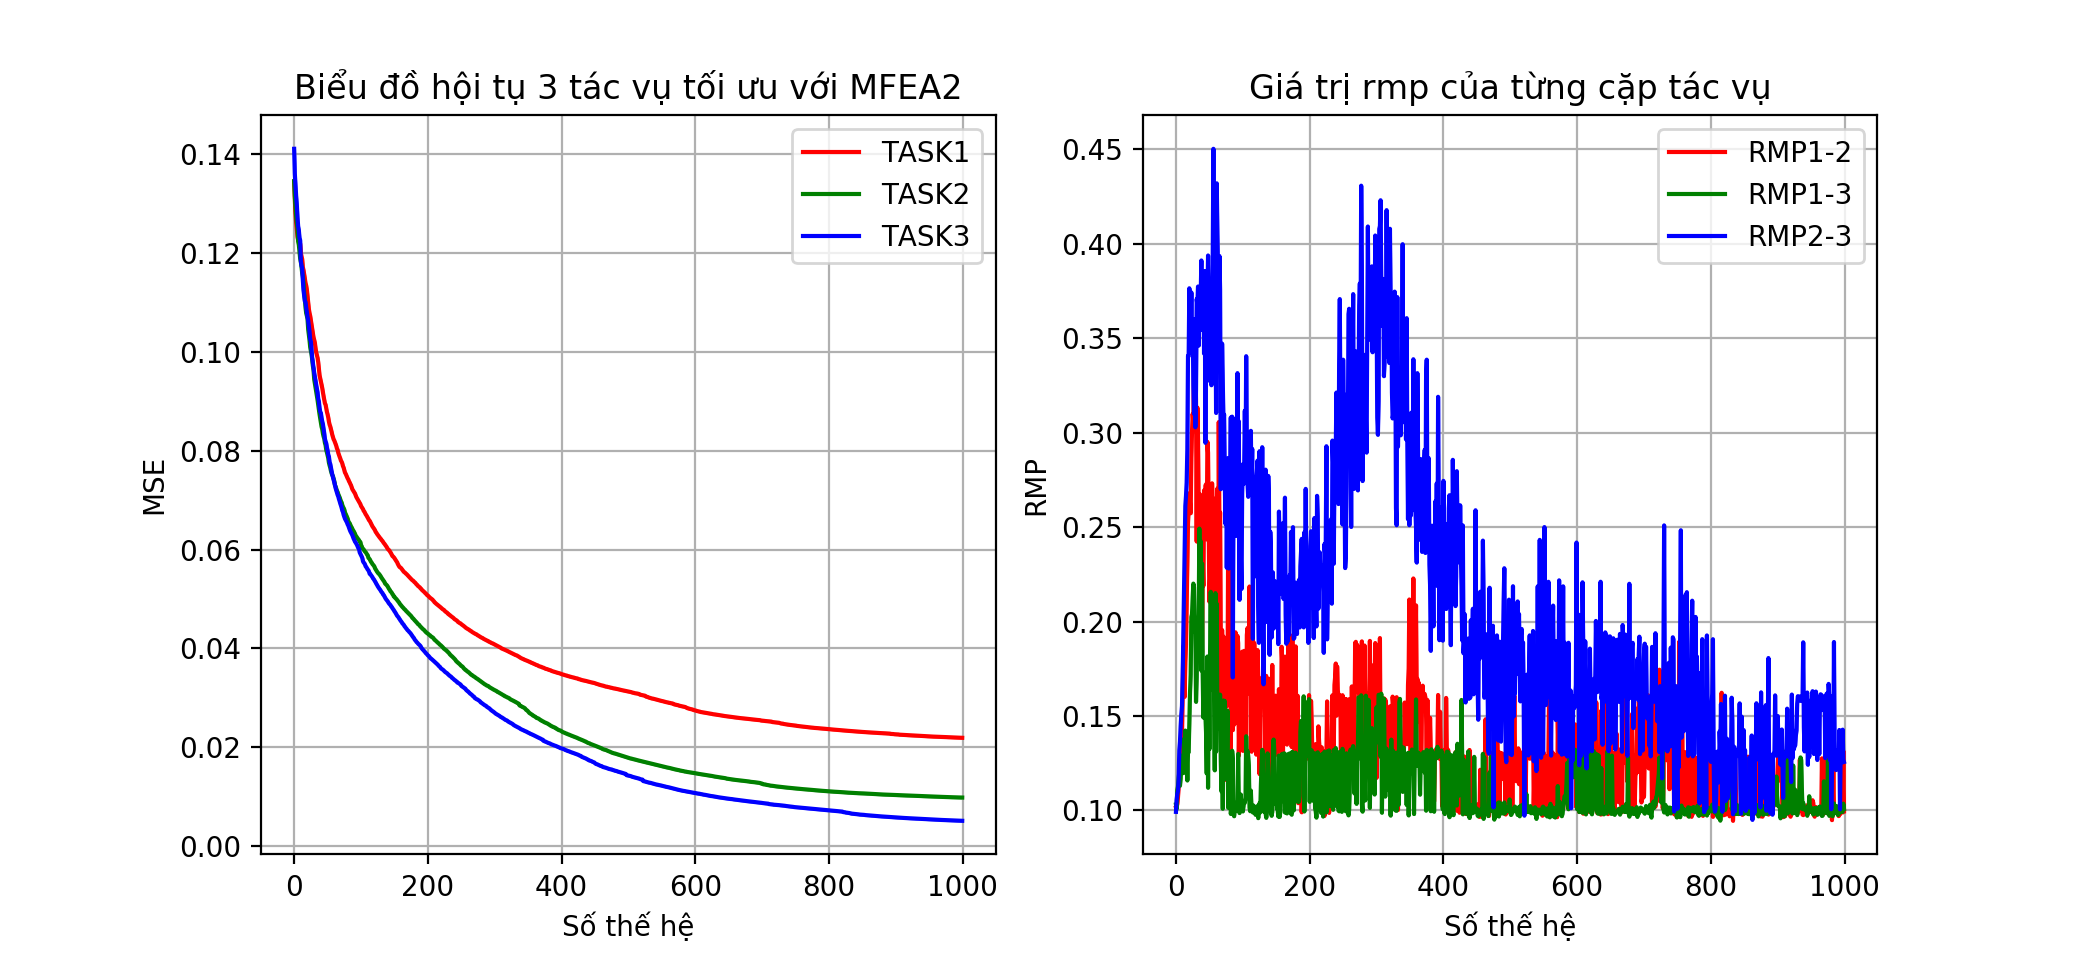
\includegraphics[width=\textwidth,height=\textheight,keepaspectratio]{images/results/nbit_1layer/4bit_rmp.png}}
            \caption{Bài 4bit: Biểu đồ tương quan giá trị rmp giữa các cặp tác vụ và hội tụ của từng tác vụ với MFEA2}
            \label{fig:my_label}
        \end{figure}
    \end{frame}
    \begin{frame}{Bài 6bit}
        \begin{columns}
            \column{0.5\textwidth}
            \begin{figure}[H]
                \centering
                \scalebox{.9}{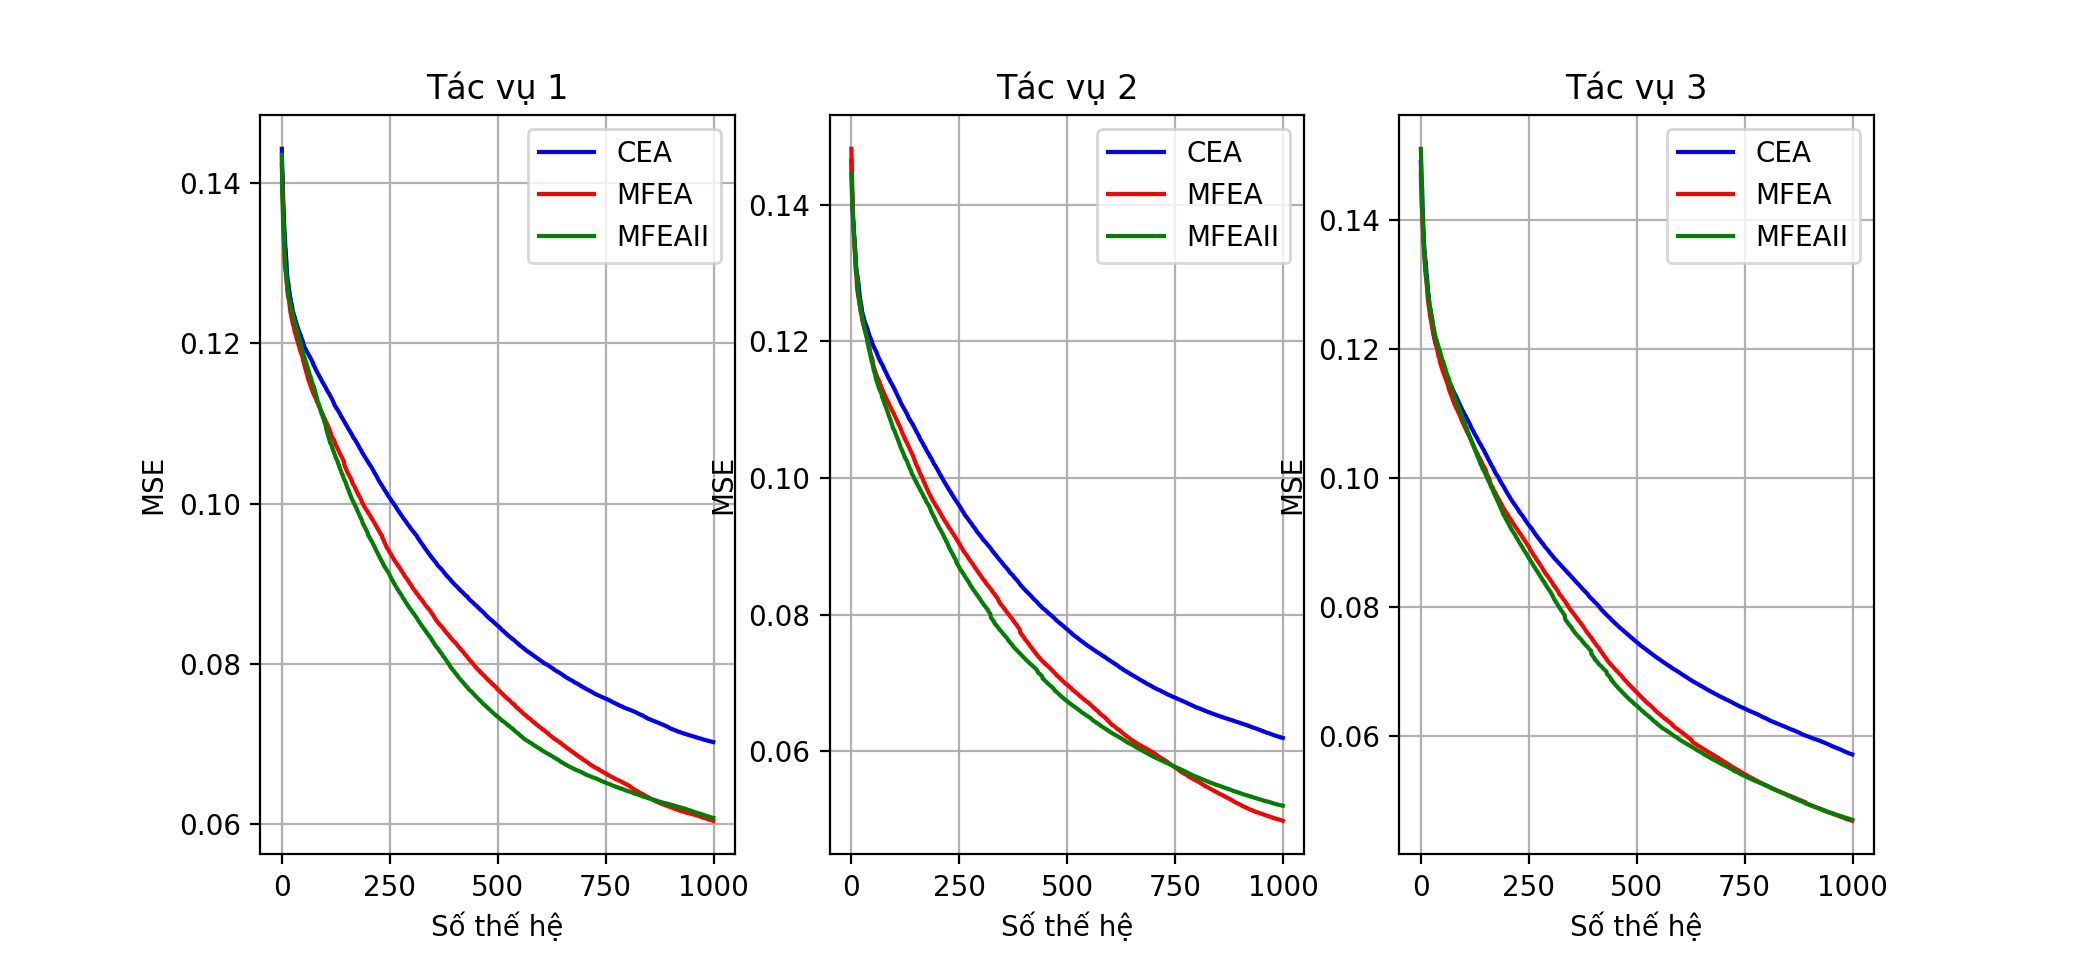
\includegraphics[width=\textwidth,height=\textheight,keepaspectratio]{images/results/nbit_1layer/6bit1_task.png}}
                \scalebox{.9}{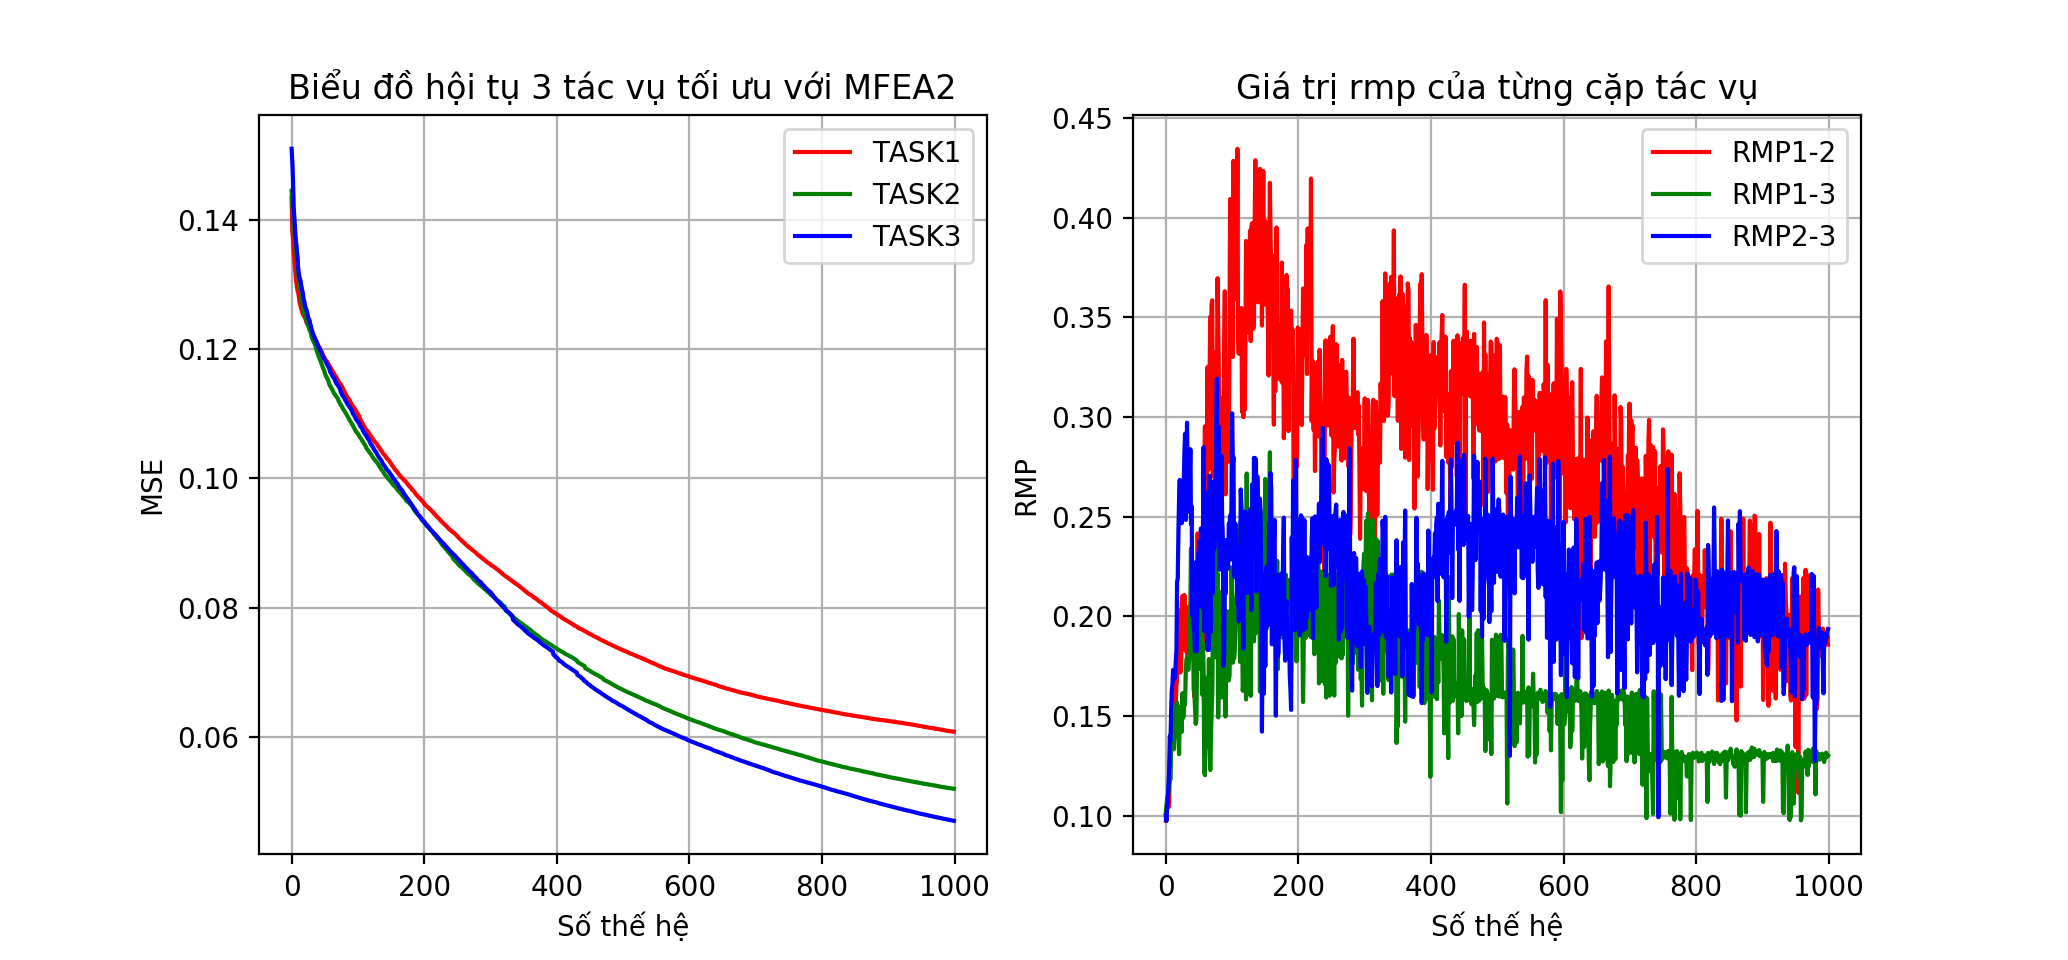
\includegraphics[width=\textwidth,height=\textheight,keepaspectratio]{images/results/nbit_1layer/6bit1_rmp.png}}
                \caption{Bài 6bit(5,6,7): Biểu đồ tương quan giá trị rmp giữa các cặp tác vụ và hội tụ của từng tác vụ với MFEA2}
                \label{fig:my_label}
            \end{figure}
            \column{0.5\textwidth}
            \begin{figure}[H]
                \centering
                \scalebox{.9}{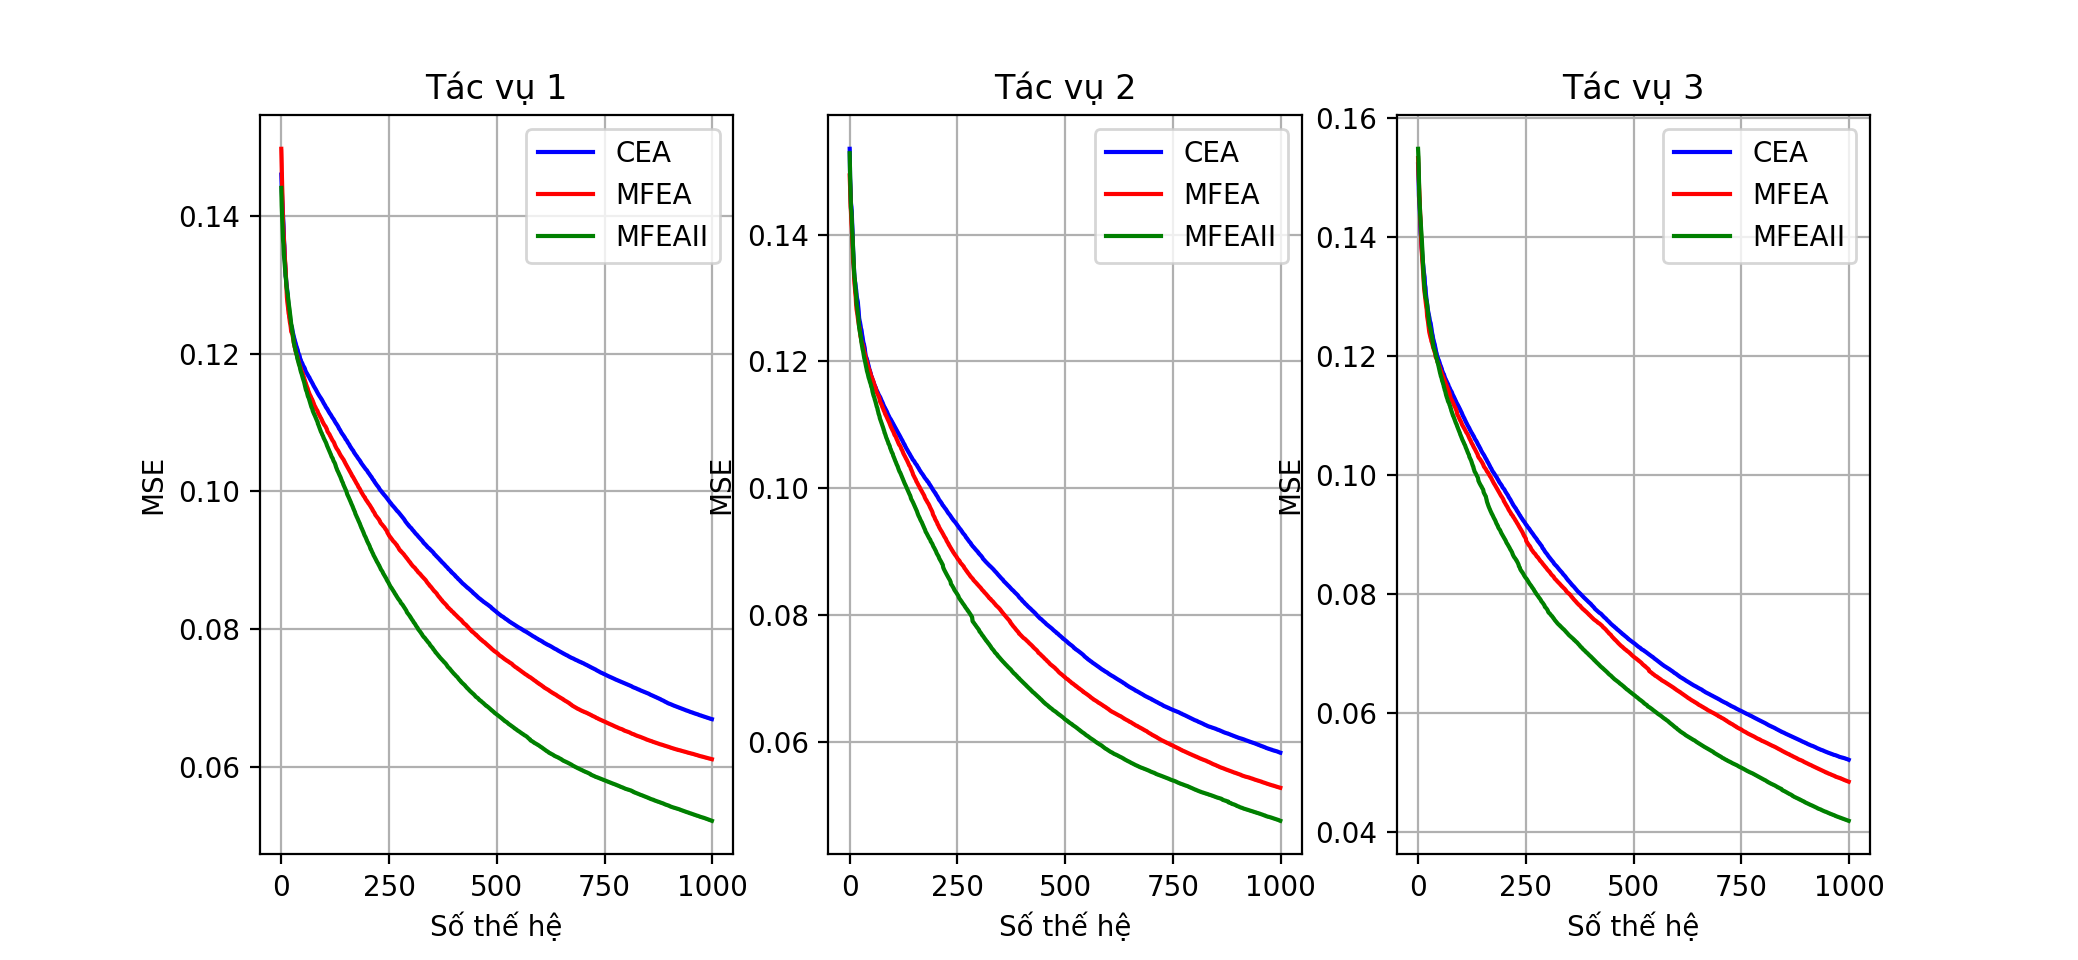
\includegraphics[width=\textwidth,height=\textheight,keepaspectratio]{images/results/nbit_1layer/6bit2_task.png}}
                \scalebox{.9}{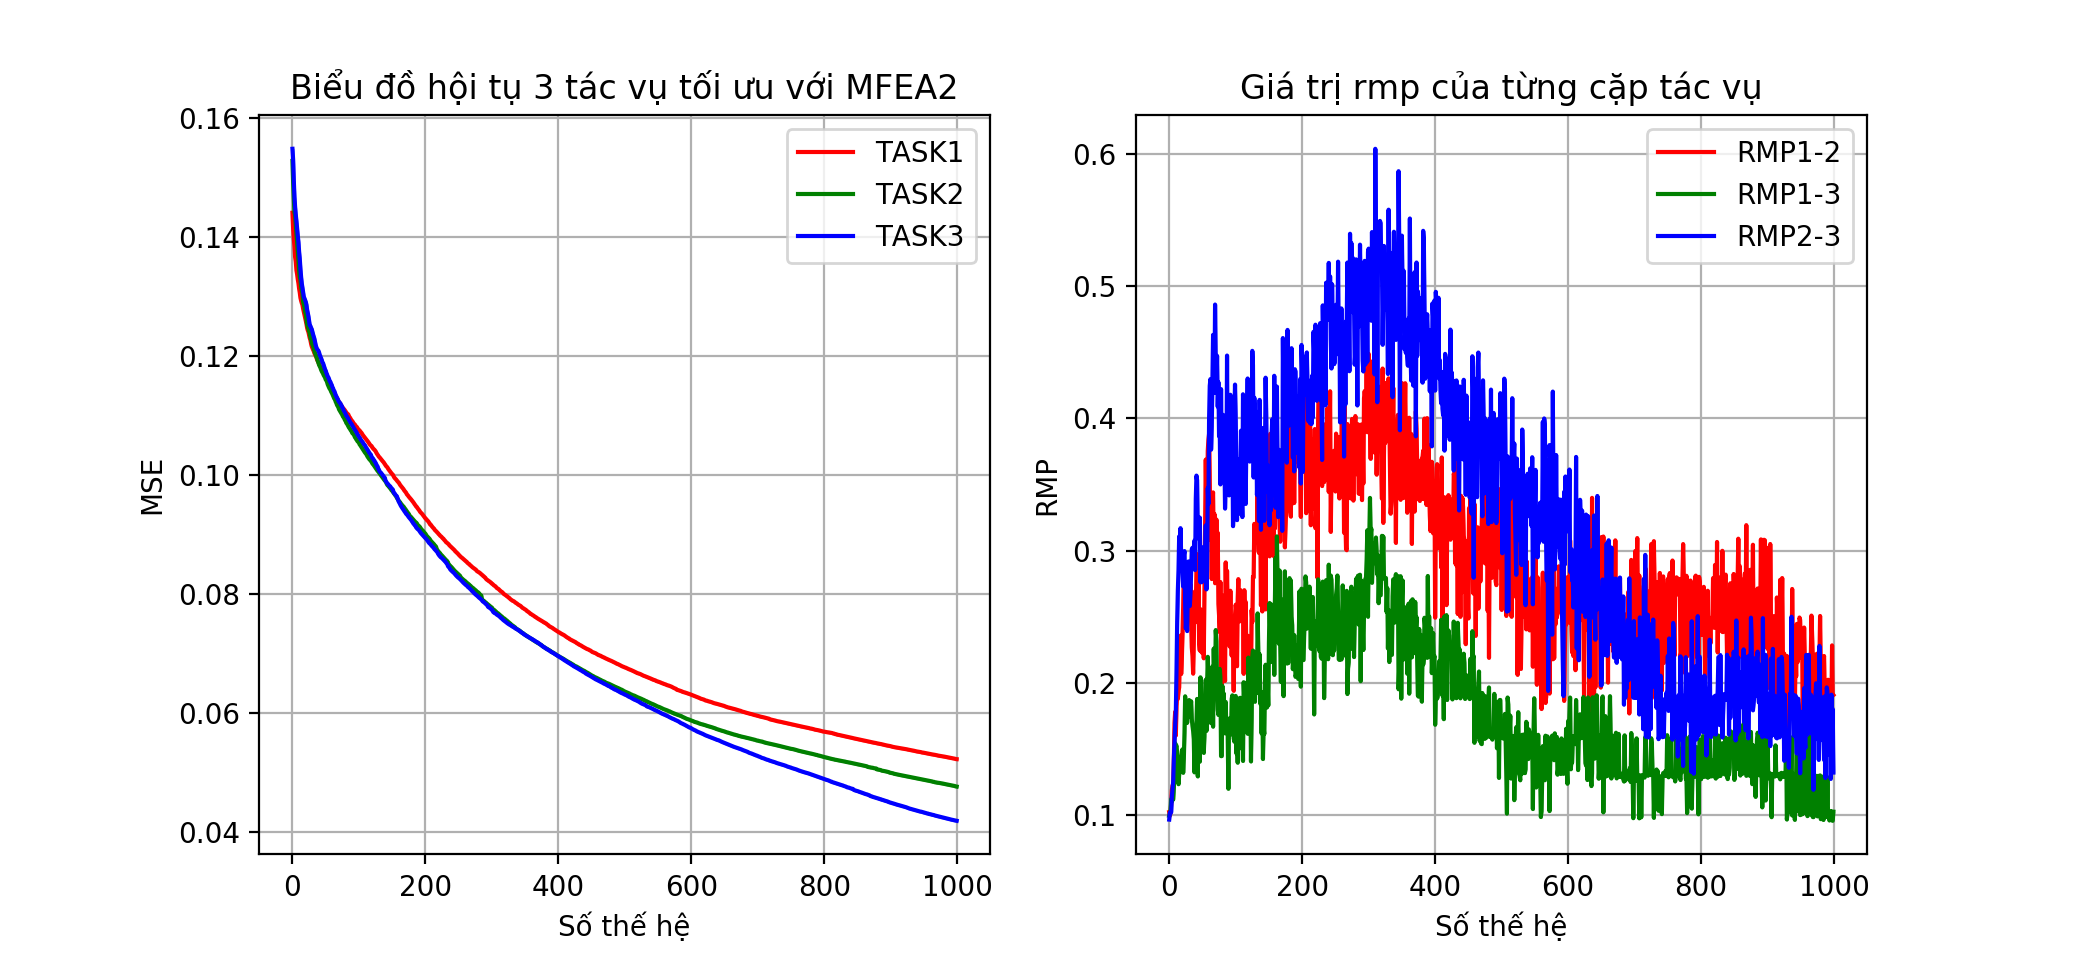
\includegraphics[width=\textwidth,height=\textheight,keepaspectratio]{images/results/nbit_1layer/6bit2_rmp.png}}
                \caption{Bài 6bit(6,7,8): Biểu đồ tương quan giá trị rmp giữa các cặp tác vụ và hội tụ của từng tác vụ với MFEA2}
                \label{fig:my_label}
            \end{figure}
        \end{columns}
    \end{frame}
    \begin{frame}{Bài 8bit}
        \begin{columns}
            \column{0.5\textwidth}
            \begin{figure}[H]
                \centering
                \scalebox{.9}{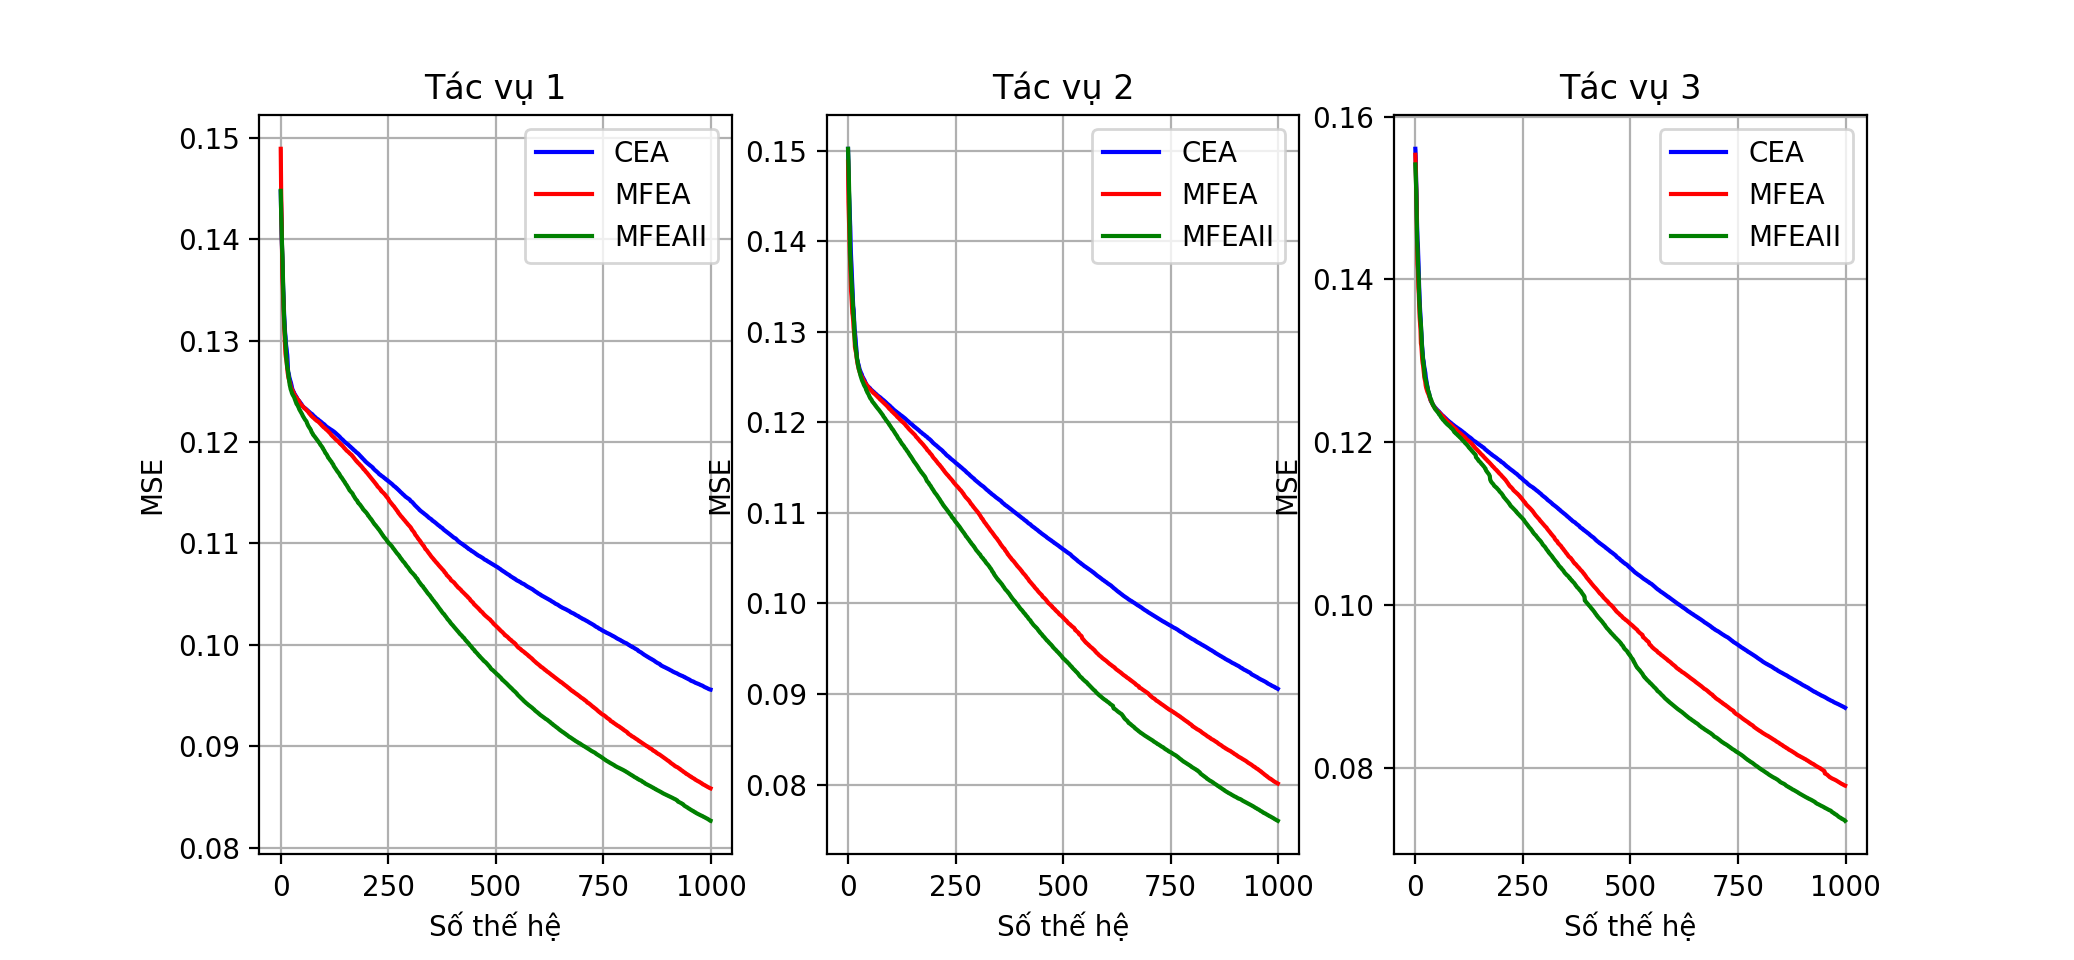
\includegraphics[width=\textwidth,height=\textheight,keepaspectratio]{images/results/nbit_1layer/8bit1_task.png}}
                \scalebox{.9}{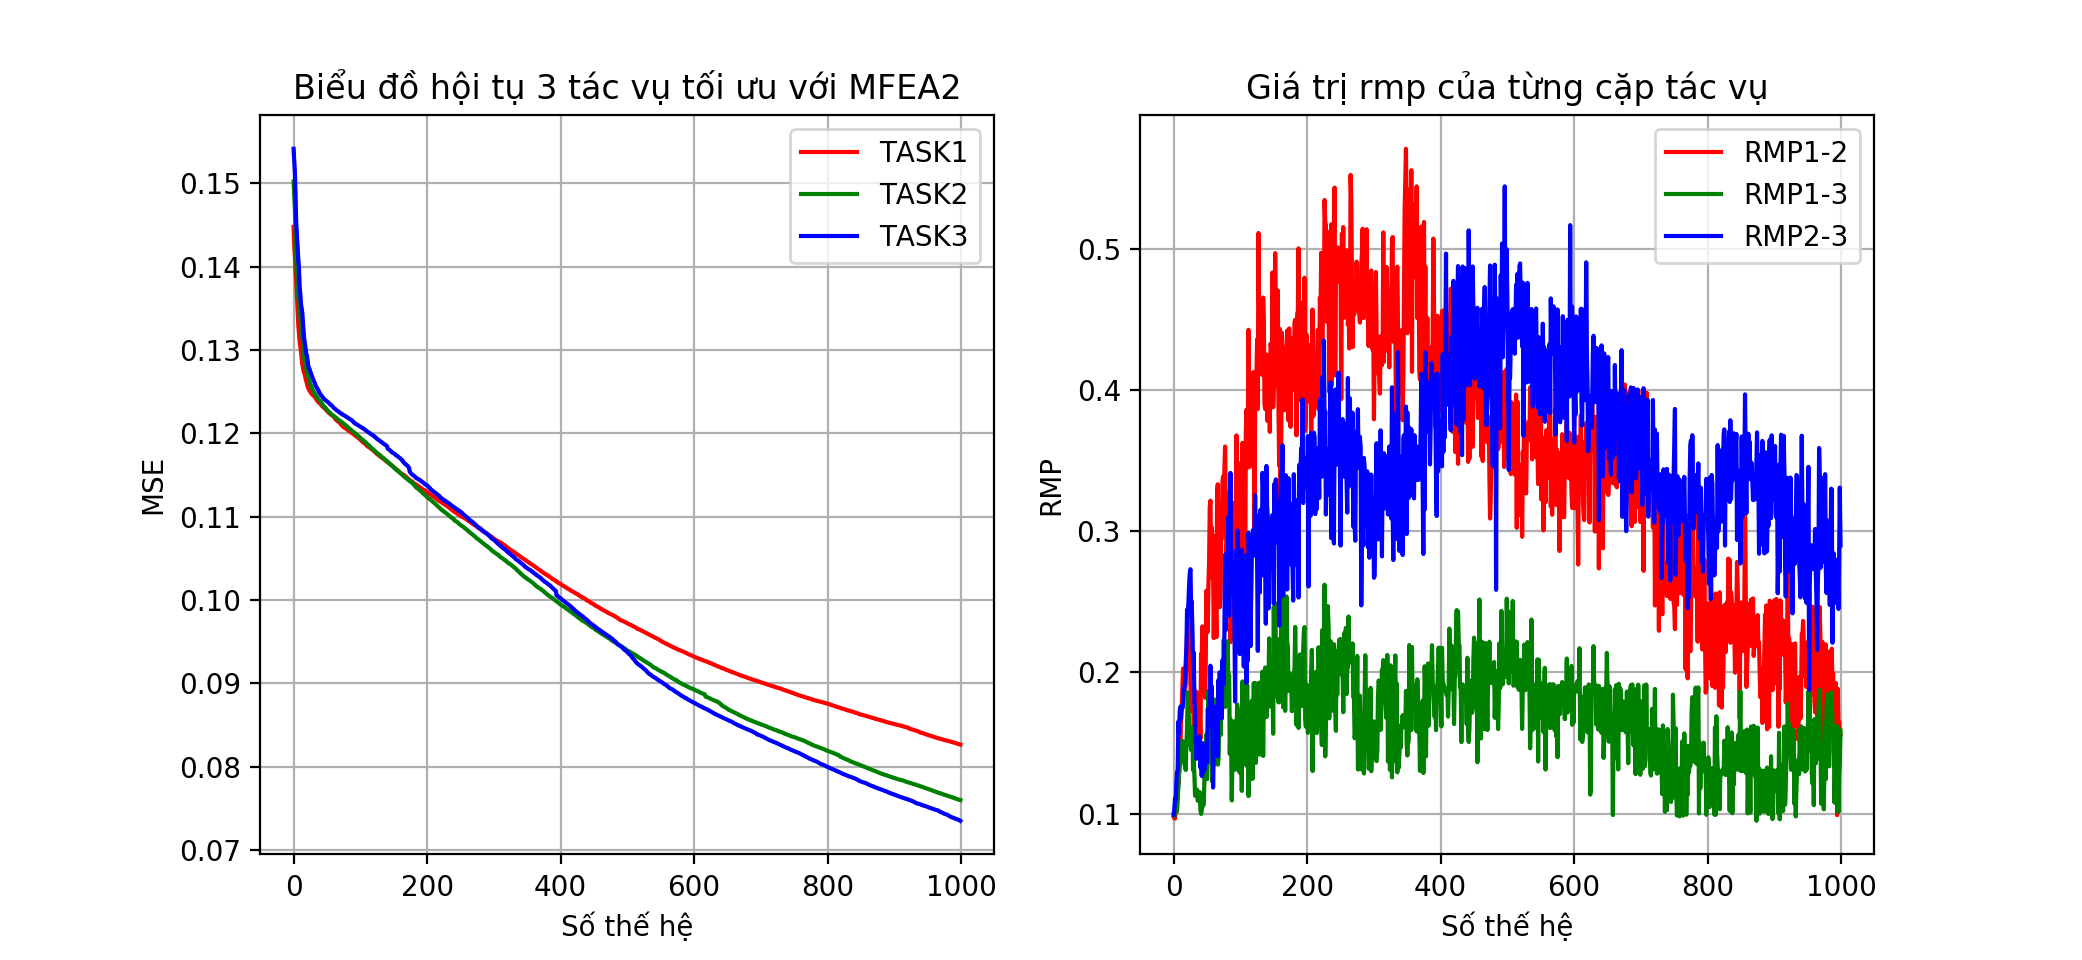
\includegraphics[width=\textwidth,height=\textheight,keepaspectratio]{images/results/nbit_1layer/8bit1_rmp.png}}
                \caption{Bài 8bit(5,6,7): Biểu đồ tương quan giá trị rmp giữa các cặp tác vụ và hội tụ của từng tác vụ với MFEA2}
                \label{fig:my_label}
            \end{figure}
            \column{0.5\textwidth}
            \begin{figure}[H]
            \centering
            \scalebox{.9}{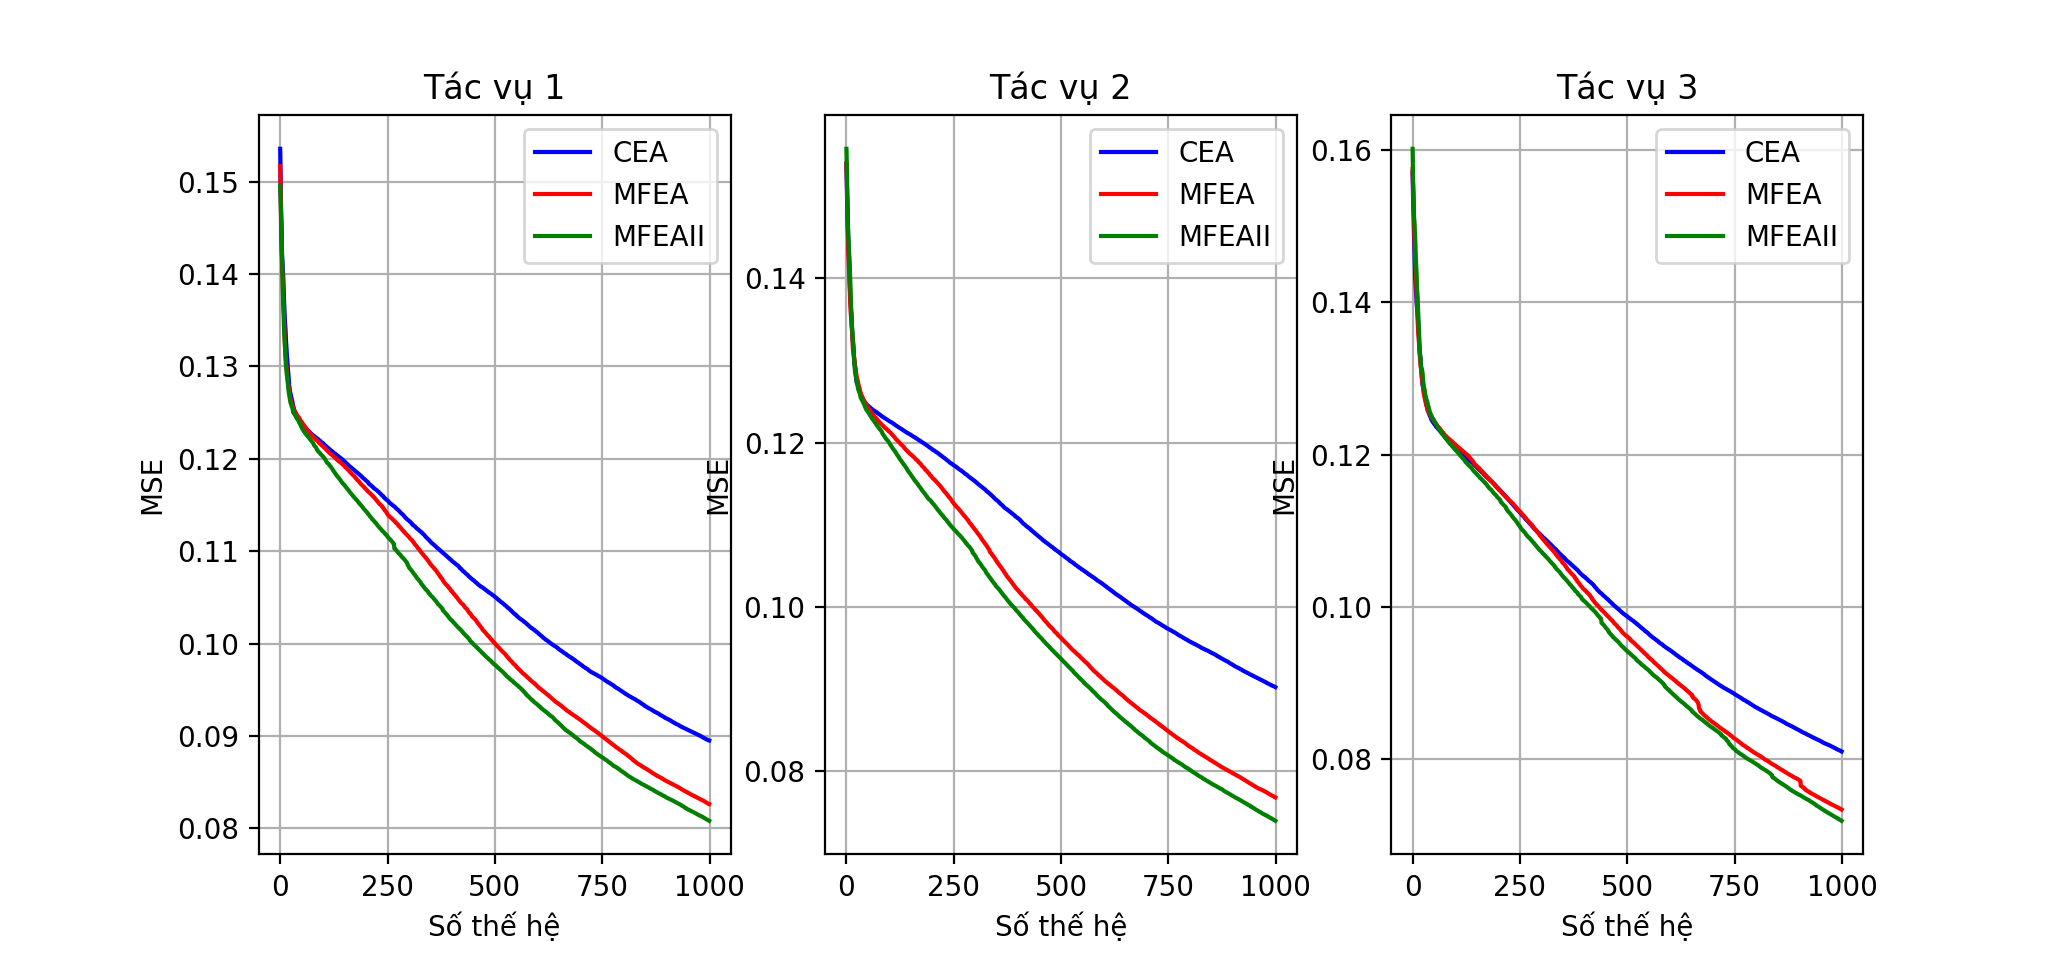
\includegraphics[width=\textwidth,height=\textheight,keepaspectratio]{images/results/nbit_1layer/8bit2_task.png}}
            \scalebox{.9}{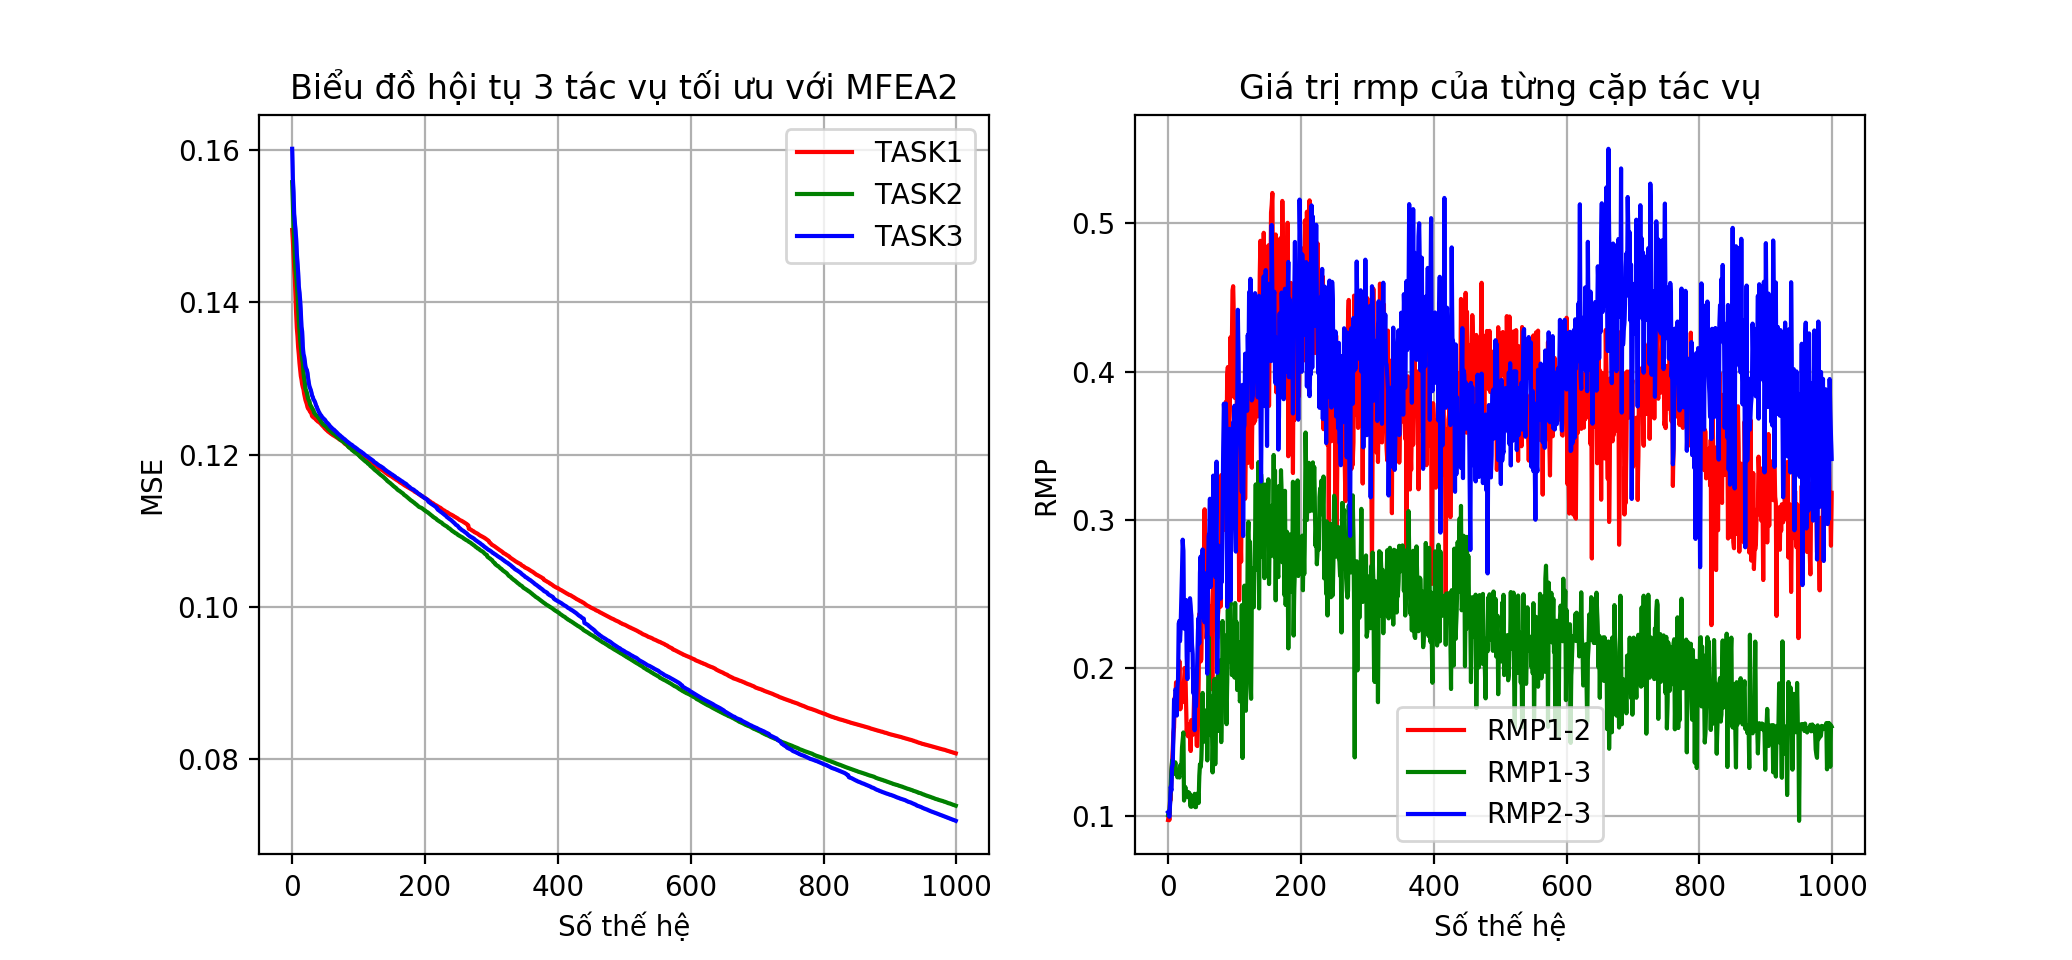
\includegraphics[width=\textwidth,height=\textheight,keepaspectratio]{images/results/nbit_1layer/8bit2_rmp.png}}
            \caption{Bài 8bit(6,7,8): Biểu đồ tương quan giá trị rmp giữa các cặp tác vụ và hội tụ của từng tác vụ với MFEA2}
            \label{fig:my_label}
        \end{figure}
        \end{columns}
    \end{frame}
    
    
    \begin{frame}{Mạng ANN 2 lớp ẩn}
        \begin{table} [H]
        \caption{Thực nghiệm kết quả mạng ANN 2 lớp ẩn}
        \begin{center}
        \begin{tabular}{|c|c|c|c|c|}
        \hline
        \multirow{1}{*}{\textbf{Bài toán}} &
        \multirow{1}{*}{\textbf{Method}} & \multicolumn{1}{c|}{\textbf{Tác vụ 1}} & \multicolumn{1}{c|}{\textbf{Tác vụ 2}} & \multicolumn{1}{c|}{\textbf{Tác vụ 3}} \\ \hline
        \multirow{3}{*} 
        {8-bit} &
        CEA & $0.075 \pm 0.012865$ & $0.0713 \pm 0.013116$ & $0.0718 \pm 0.012432$  \\
        & MFEA-I & $0.0738 \pm 0.012508$ & $0.0684 \pm 0.013252$ & $0.0669 \pm 0.015076$   \\
        & MFEA-II & $\mathbf{0.0705 \pm 0.012856}$ & $\mathbf{0.0624 \pm 0.011079}$ & $\mathbf{0.0595 \pm 0.011252}$\\\hline
        \multirow{3}{*} 
        {9-bit} &
        CEA & $0.0826 \pm 0.010588$ & $0.0751 \pm 0.014406$ & $0.0785 \pm 0.010766$  \\
        & MFEA-I & $0.0827 \pm 0.010438$ & $0.0762 \pm 0.009495$ & $0.0737 \pm 0.009766$ \\
        & MFEA-II & $\mathbf{0.0795 \pm 0.012865}$ & $\mathbf{0.0705 \pm 0.009581}$ & $\mathbf{0.0685 \pm 0.011156}$ \\\hline
        \multirow{3}{*} 
        {10-bit} &
        CEA & $0.0853 \pm 0.01105$ & $0.0862 \pm 0.008326$ & $0.0856 \pm 0.008919$  \\
        & MFEA-I  & $0.0855 \pm 0.012229$ & $\mathbf{0.0782 \pm 0.009659}$ & $\mathbf{0.0752 \pm 0.009681}$ \\
        & MFEA-II & $\mathbf{0.0833 \pm 0.010222}$ & $0.0791 \pm 0.009846$ & $0.0762 \pm 0.010419$ \\\hline
        \end{tabular}
        \end{center}
        
        \label{tab:result:nbit}
        \end{table}
    \end{frame}
    \begin{frame}{Mạng nơ-ron khác độ sâu}
        \begin{table} [H]
    \caption{Mạng ANN khác độ sâu}
    \begin{center}
    \begin{tabular}{|c|c|c|c|c|}
    \hline
    \multirow{1}{*}{\textbf{Bài toán}} &
    \multirow{1}{*}{\textbf{Method}} & \multicolumn{1}{c|}{\textbf{Tác vụ 1}} & \multicolumn{1}{c|}{\textbf{Tác vụ 2}} & \multicolumn{1}{c|}{\textbf{Tác vụ 3}} \\ \hline
    \multirow{3}{*} 
    {8-bit} &
    CEA & $0.0843 \pm 0.016042$ & $0.0842 \pm 0.014995$ & $0.0892 \pm 0.007818$ \\
    & MFEA-I & $\mathbf{0.0775 \pm 0.014683}$ & $0.0797 \pm 0.009343$ & $0.0812 \pm 0.017086$  \\
    & MFEA-II & $0.0837 \pm 0.021442$ & $\mathbf{0.0732 \pm 0.014932}$ & $\mathbf{0.0738 \pm 0.013425}$\\\hline
    \multirow{3}{*} 
    {9-bit} &
    CEA & $0.0916 \pm 0.009395$ & $0.0869 \pm 0.010216$ & $\mathbf{0.0786 \pm 0.010333}$ \\
    & MFEA-I  & $0.0858 \pm 0.01389$ & $0.0841 \pm 0.016001$ & $0.0794 \pm 0.015452$ \\
    & MFEA-II & $\mathbf{0.0845 \pm 0.009553}$ & $\mathbf{0.0827 \pm 0.010715}$ & $0.0889 \pm 0.011707$ \\\hline
    \multirow{3}{*} 
    {10-bit} &
    CEA & $0.0905 \pm 0.006423$ & $0.0901 \pm 0.015163$ & $0.0918 \pm 0.008761$  \\
    & MFEA-I  & $0.0917 \pm 0.006814$ & $0.0844 \pm 0.013841$ & $\mathbf{0.0861 \pm 0.009332}$ \\
    & MFEA-II & $\mathbf{0.0816 \pm 0.009981}$ & $\mathbf{0.0815 \pm 0.012087}$ & $0.0871 \pm 0.009619$ \\\hline
    \end{tabular}
    \end{center}
    
    \label{tab:result:nbit}
\end{table}

    \end{frame}
    \begin{frame}{Biểu đồ hội tụ bài cùng độ sâu}
        \begin{columns}
            \column{0.5\textwidth}
            \begin{figure}[H]
                \centering
                \scalebox{.9}{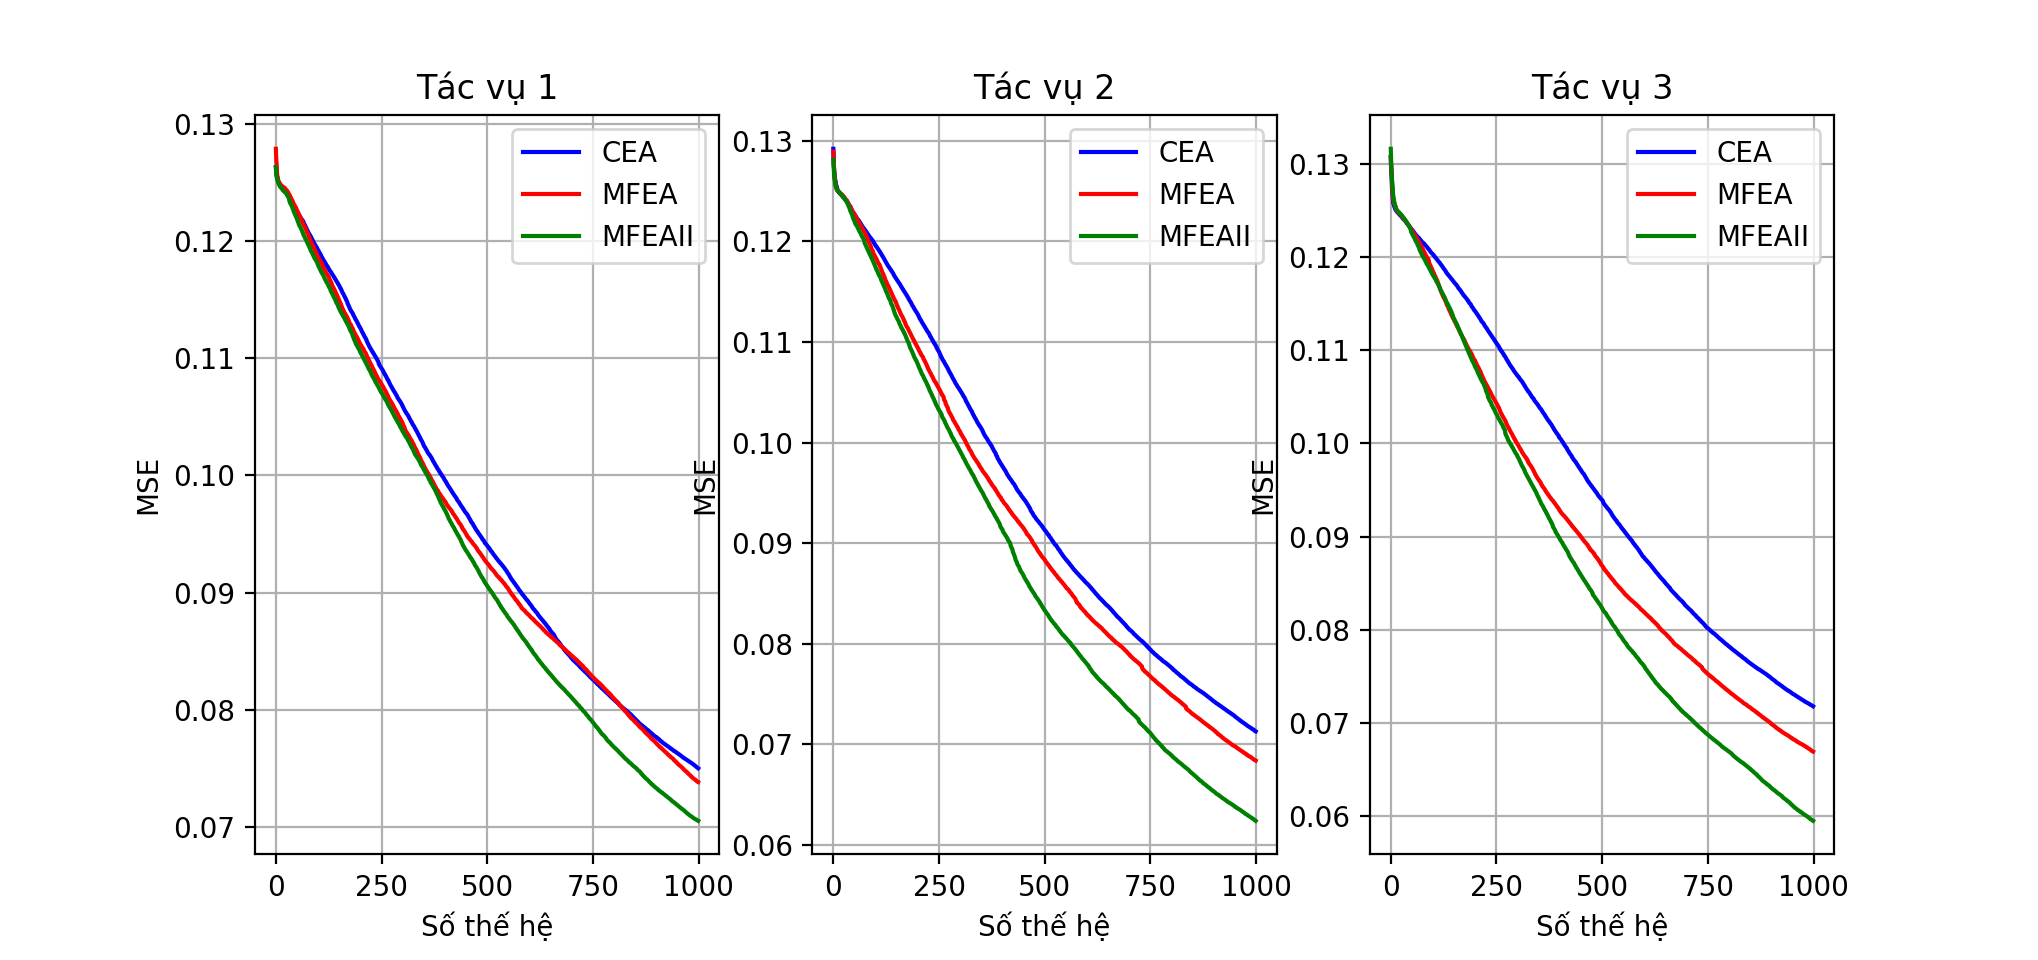
\includegraphics[width=\textwidth,height=\textheight,keepaspectratio]{images/results/nbit_2layer/8bit1_task.png}}
                \scalebox{.9}{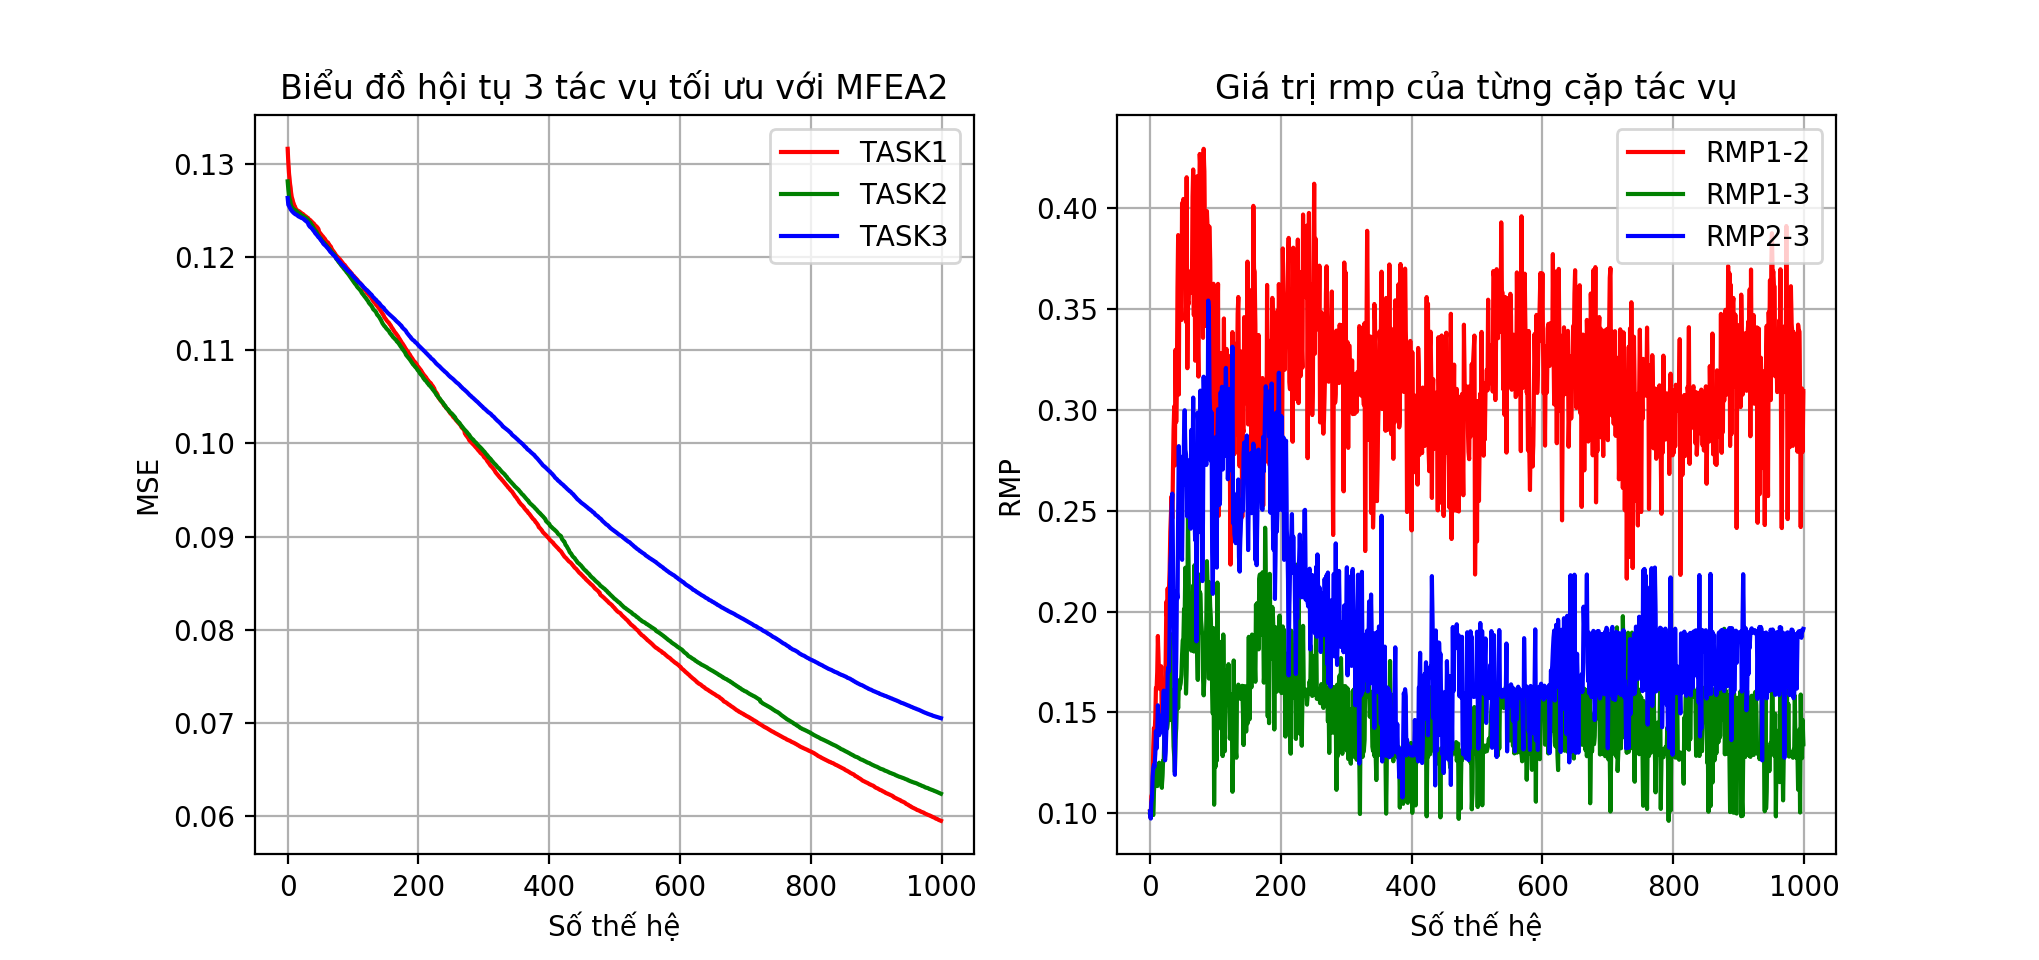
\includegraphics[width=\textwidth,height=\textheight,keepaspectratio]{images/results/nbit_2layer/8bit1_rmp.png}}
                \caption{Bài 8-bit: Biểu đồ tương quan giá trị rmp giữa các cặp tác vụ và hội tụ của từng tác vụ với MFEA2}
                \label{fig:my_label}
            \end{figure}
            \column{0.5\textwidth}
            \begin{figure}[H]
            \centering
            \scalebox{.9}{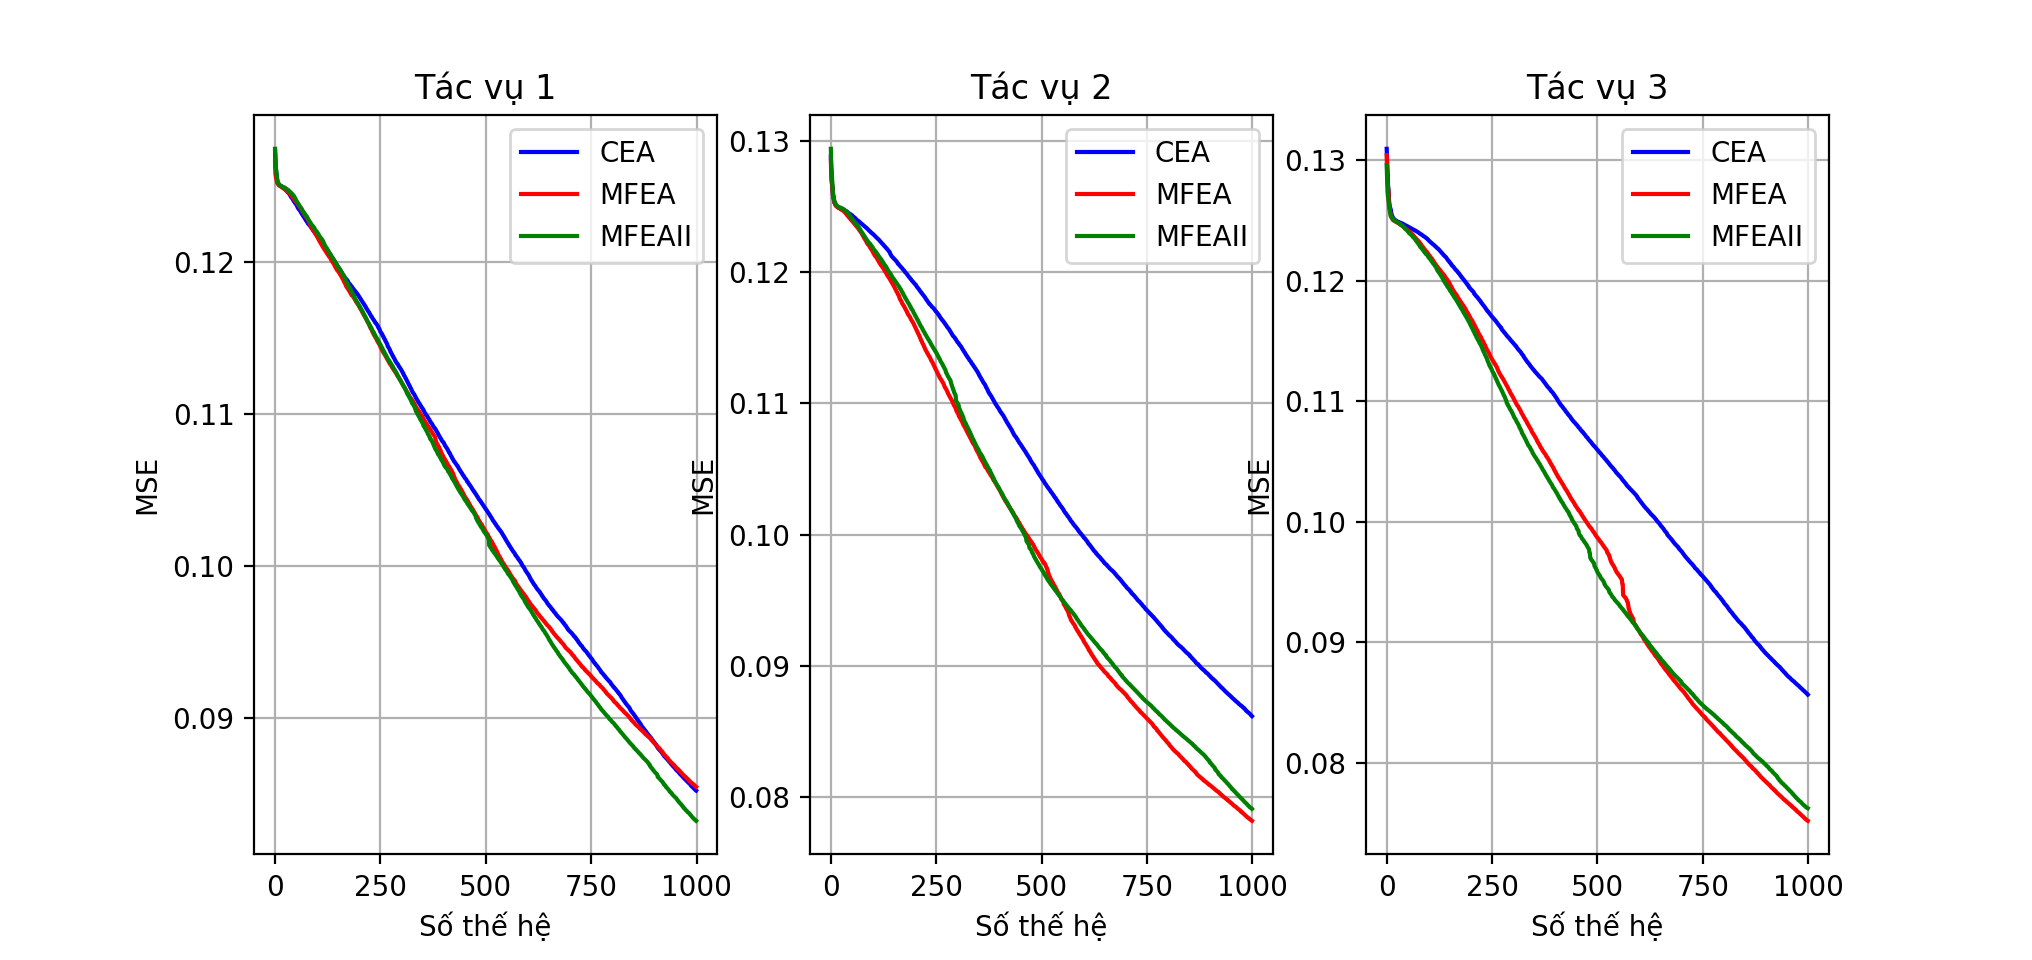
\includegraphics[width=\textwidth,height=\textheight,keepaspectratio]{images/results/nbit_2layer/10bit1_task.png}}
            \scalebox{.9}{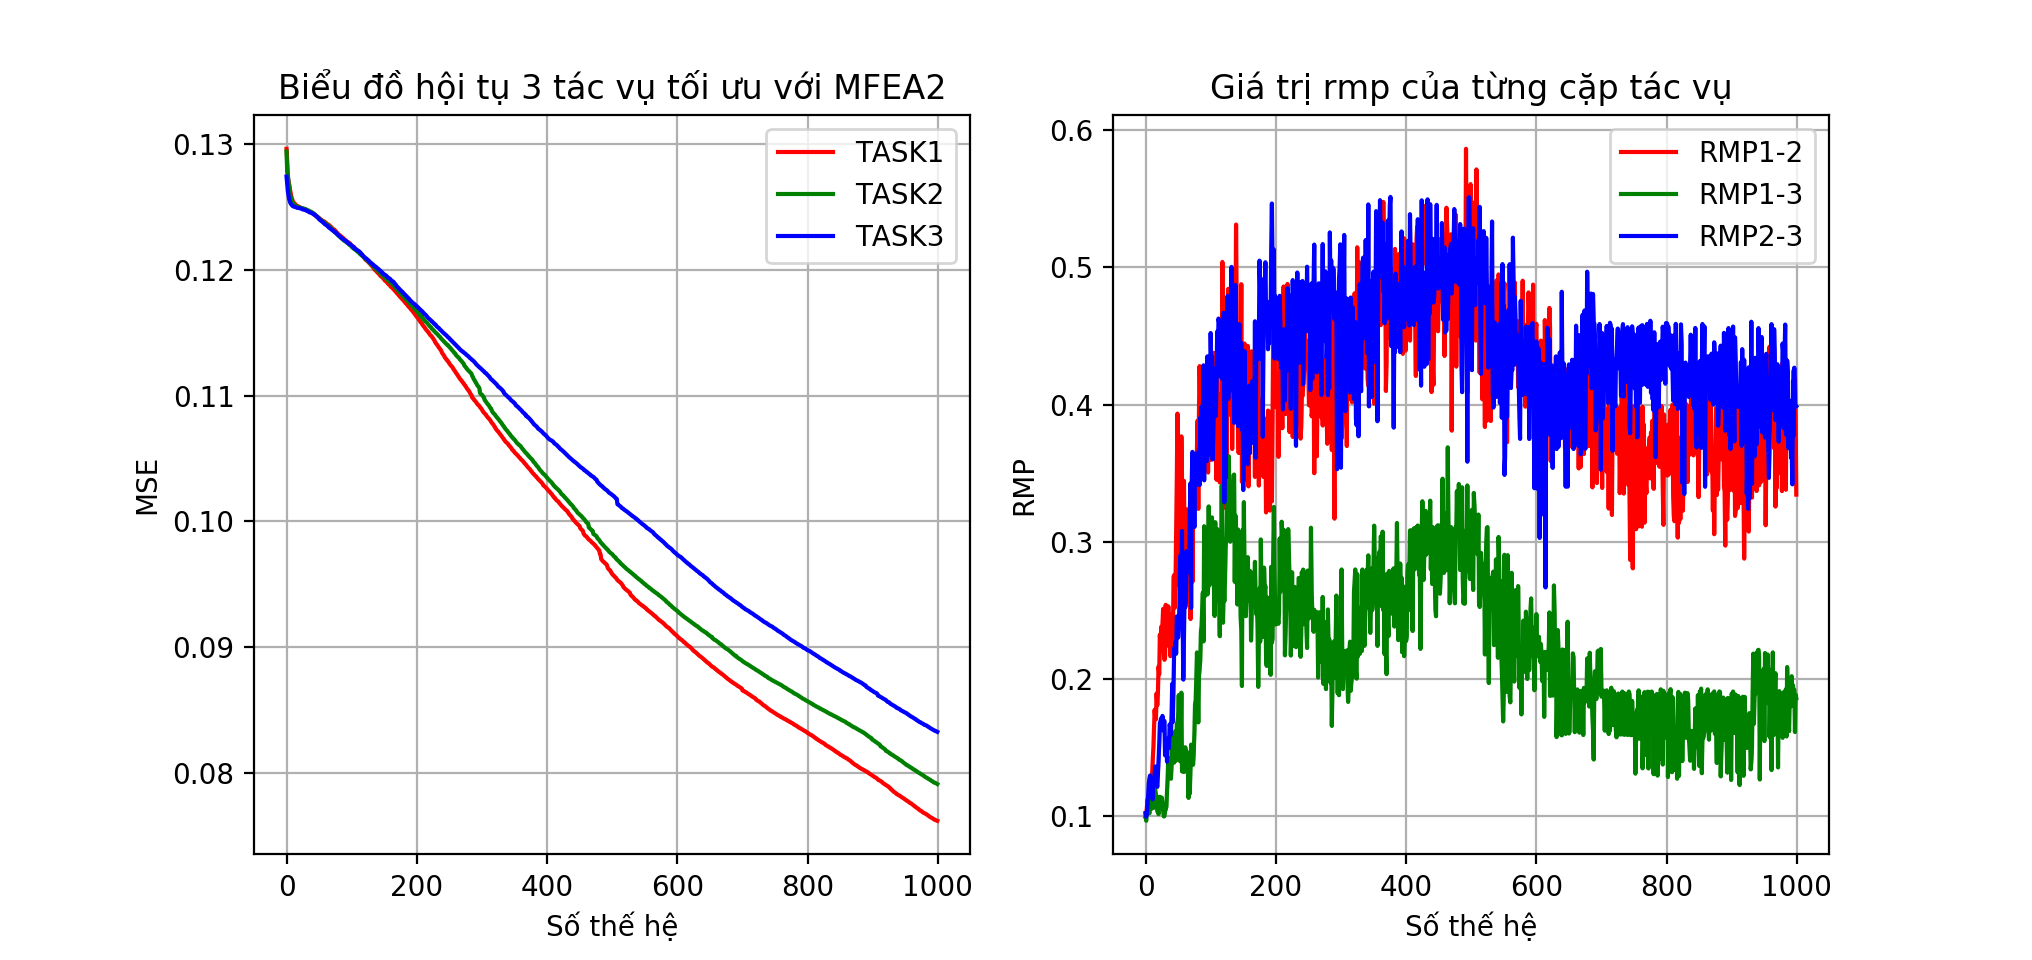
\includegraphics[width=\textwidth,height=\textheight,keepaspectratio]{images/results/nbit_2layer/10bit1_rmp.png}}
            \caption{Bài 10-bit: Biểu đồ tương quan giá trị rmp giữa các cặp tác vụ và hội tụ của từng tác vụ với MFEA2}
            \label{fig:my_label}
        \end{figure}
        \end{columns}
    \end{frame}
    \begin{frame}{UCI cùng đo}
    \begin{table}[h!]
        \begin{tabular}{|c|c|c|c|c|}
        \hline
        \multirow{1}{*}{\textbf{Instance}} & \multicolumn{1}{c|} {\textbf{Method}} & \multicolumn{1}{c|}{\textbf{Subtask1}} & \multicolumn{1}{c|}{\textbf{Subtask 2}} & \multicolumn{1}{c|}{\textbf{Subtask 3}} \\ \hline
        \multirow{3}{*} 
        {breastCancer} & CEA & $0.0097 \pm 0.0012$ & $0.0092 \pm 0.0007$ & $0.0093 \pm 0.0009$ \\
         & MFEA-I & $0.0097 \pm 0.0006$ & $0.0093 \pm 0.0005$ & $0.0091 \pm 0.0005$ \\ 
        & MFEA II & $\mathbf{0.0094 \pm 0.0008}$ & $\mathbf{0.0089 \pm 0.0006}$ & $\mathbf{0.0087 \pm 0.0004}$ \\ \hline
        \multirow{3}{*} {creditScreening} & CEA & $0.0509 \pm 0.0033$ & $0.0514 \pm 0.0033$ & $0.0508 \pm 0.004$ \\
       & MFEA-I & $0.0504 \pm 0.0024$ & $0.0503 \pm 0.0025$ & $0.0513 \pm 0.0022$ \\ 
       & MFEA-II & $\mathbf{0.0492 \pm 0.0023}$ & $\mathbf{0.0489 \pm 0.002}$ & $\mathbf{0.0491 \pm 0.002}$ \\ \hline
        \multirow{3}{*} {ionosphere} & CEA & $0.0384 \pm 0.0072$ & $0.0389 \pm 0.0129$ & $0.035 \pm 0.0047$ \\
        &MFEA-I & $0.0367 \pm 0.0068$ & $0.0347 \pm 0.0075$ & $0.0351 \pm 0.0088$ \\
        &MFEA-II & $\mathbf{0.0343 \pm 0.0079}$ & $\mathbf{0.0322 \pm 0.0071}$ & $\mathbf{0.032 \pm 0.007}$ \\\hline
        \multirow{3}{*} {ticTacToe} & CEA & $0.089 \pm 0.0047$ & $0.0838 \pm 0.0054$ & $0.0869 \pm 0.0049$ \\
        &MFEA-I & $0.0845 \pm 0.0049$ & $0.0818 \pm 0.0047$ & $0.0824 \pm 0.0047$ \\
        &MFEA-II & $\mathbf{0.082 \pm 0.0048}$ & $\mathbf{0.0815 \pm 0.0046}$ & $\mathbf{0.0812 \pm 0.0043}$  \\\hline
        
        \end{tabular}
    
        \label{tab:result:nbit}
        \caption{Huấn luyện nhiều ANN trên bộ dữ liệu UCI cùng độ sâu}
    \end{table}
    \end{frame}
    
    \begin{frame}{Khác độ sâu UCI}
        \begin{table}[h!]
        \begin{tabular}{|c|c|c|c|c|}
        \hline
        \multirow{1}{*}{\textbf{Instance}} & \multicolumn{1}{c|} {\textbf{Method}} & \multicolumn{1}{c|}{\textbf{Subtask1}} & \multicolumn{1}{c|}{\textbf{Subtask 2}} & \multicolumn{1}{c|}{\textbf{Subtask 3}} \\ \hline
        \multirow{3}{*} 
        {breastCancer} & CEA & $0.0119 \pm 0.0029$ & $0.0107 \pm 0.002$ & $\mathbf{0.0093 \pm 0.0005}$ \\
         & MFEA-I & $\mathbf{0.011 \pm 0.0015}$ & $0.0102 \pm 0.0012$ & $0.0094 \pm 0.0005$  \\ 
        & MFEA II & $\mathbf{0.011 \pm 0.0015}$ & $\mathbf{0.01 \pm 0.0011}$ & $0.0096 \pm 0.0011$ \\ \hline
        
        \multirow{3}{*} {creditScreening} & CEA & $0.054 \pm 0.0071$ & $0.0503 \pm 0.0027$ & $0.0485 \pm 0.0017$ \\
       & MFEA-I & $\mathbf{0.0508 \pm 0.0023}$ & $0.0497 \pm 0.0019$ & $0.0496 \pm 0.0021$ \\ 
       & MFEA-II & $0.0515 \pm 0.0033$ & $\mathbf{0.0494 \pm 0.0023}$ & $\mathbf{0.0485 \pm 0.0018}$ \\ \hline
       
        \multirow{3}{*} {ionosphere} & CEA & $0.0516 \pm 0.0124$ & $0.0449 \pm 0.0114$ & $0.0366 \pm 0.0094$ \\
        &MFEA-I & $0.049 \pm 0.0131$ & $0.0413 \pm 0.0112$ & $\mathbf{0.0365 \pm 0.007}$ \\
        &MFEA-II & $\mathbf{0.0473 \pm 0.0083}$ & $\mathbf{0.0387 \pm 0.0109}$ & $0.0367 \pm 0.008$  \\\hline
        
        \multirow{3}{*} {ticTacToe} & CEA & $0.0899 \pm 0.0067$ & $0.0879 \pm 0.0079$ & $0.0852 \pm 0.0045$  \\
        &MFEA-I & $\mathbf{0.088 \pm 0.008}$ & $0.0886 \pm 0.0064$ & $0.0843 \pm 0.0092$  \\
        &MFEA-II & $\mathbf{0.088 \pm 0.0073}$ & $\mathbf{0.0832 \pm 0.0067}$ & $0\mathbf{.0817 \pm 0.0046}$  \\\hline
        
        \end{tabular}
    
        \label{tab:result:nbit}
        \caption{Huấn luyện nhiều ANN trên bộ dữ liệu UCI khác độ sâu}
    \end{table}
    \end{frame}
    
    \begin{frame}{Học tăng cường}
    \begin{table}
    \caption{Mô hình học tăng cường khác môi trường}
    \begin{center}
    \begin{tabular}{|c|c|c|c|c|c|}
    \hline
    \multirow{1}{*}{\textbf{Trọng lực}} &
    \multirow{1}{*}{\textbf{Method}} & \multicolumn{1}{c|}{\textbf{Cao nhất}} & {\textbf{Thấp nhất}} & \multicolumn{1}{c|}{\textbf{Trung Bình}} & \multicolumn{1}{c|}{\textbf{Độ lệch}} \\ \hline
    \multirow{3}{*} 
    {Trọng lực=1.0} &
    CEA & $71$ & $4$ & $28.86$ & $17.16$ \\
    & MFEA-I & $\mathbf{129}$ & $17$ &$46.71$ & $20.36$  \\
    & MFEA-II & $84$ & $15$ & $\mathbf{52.81}$  &$15.45$\\\hline
    \multirow{3}{*} 
    {Trọng lực=1.98} &
    CEA & $382$ & $7$ &$174.86$ & $113.79$ \\
    & MFEA-I  & $\mathbf{546}$ & $98$ & $\mathbf{319.86}$ & $95.34$ \\
    & MFEA-II & $517$ & $\mathbf{131}$ &$311.38$ & $106.76$ \\\hline
    \multirow{3}{*} 
    {Trọng lực=2.96} &
    CEA & $272$ & $1$ &$97.9$ & $83.07$ \\
    & MFEA-I  & $\mathbf{349}$ & $\mathbf{140}$ & $\mathbf{222.81}$ & $52.07$ \\
    & MFEA-II & $322$ & $103$ &$212.38$ & $52.74$ \\\hline
    \multirow{3}{*} 
    {Trọng lực=3.94} &
    CEA & $227$ & $2$ &$69.24$ & $56.64$ \\
    & MFEA-I  & $\mathbf{217}$ & $\mathbf{95}$ & $\mathbf{142.86}$ & $27.4$ \\
    & MFEA-II & $190$ & $76$ &$140.38$ & $27.78$ \\\hline
    \multirow{3}{*} 
    {Trọng lực=4.92} &
    CEA & $95$ & $2$ & $25.48$ & $25.78$  \\
    & MFEA-I  & $\mathbf{181}$ & $\mathbf{54}$ & $90.86$ & $21.98$ \\
    & MFEA-II & $145$ & $44$ & $\mathbf{102.14}$ & $26.66$ \\\hline
    \end{tabular}
    \end{center}
    
    \label{tab:result:nbit}
\end{table}

    \end{frame}
    \begin{frame}{So sánh mức độ phân bố kết quả}
        \begin{figure}[h!]
        \centering
        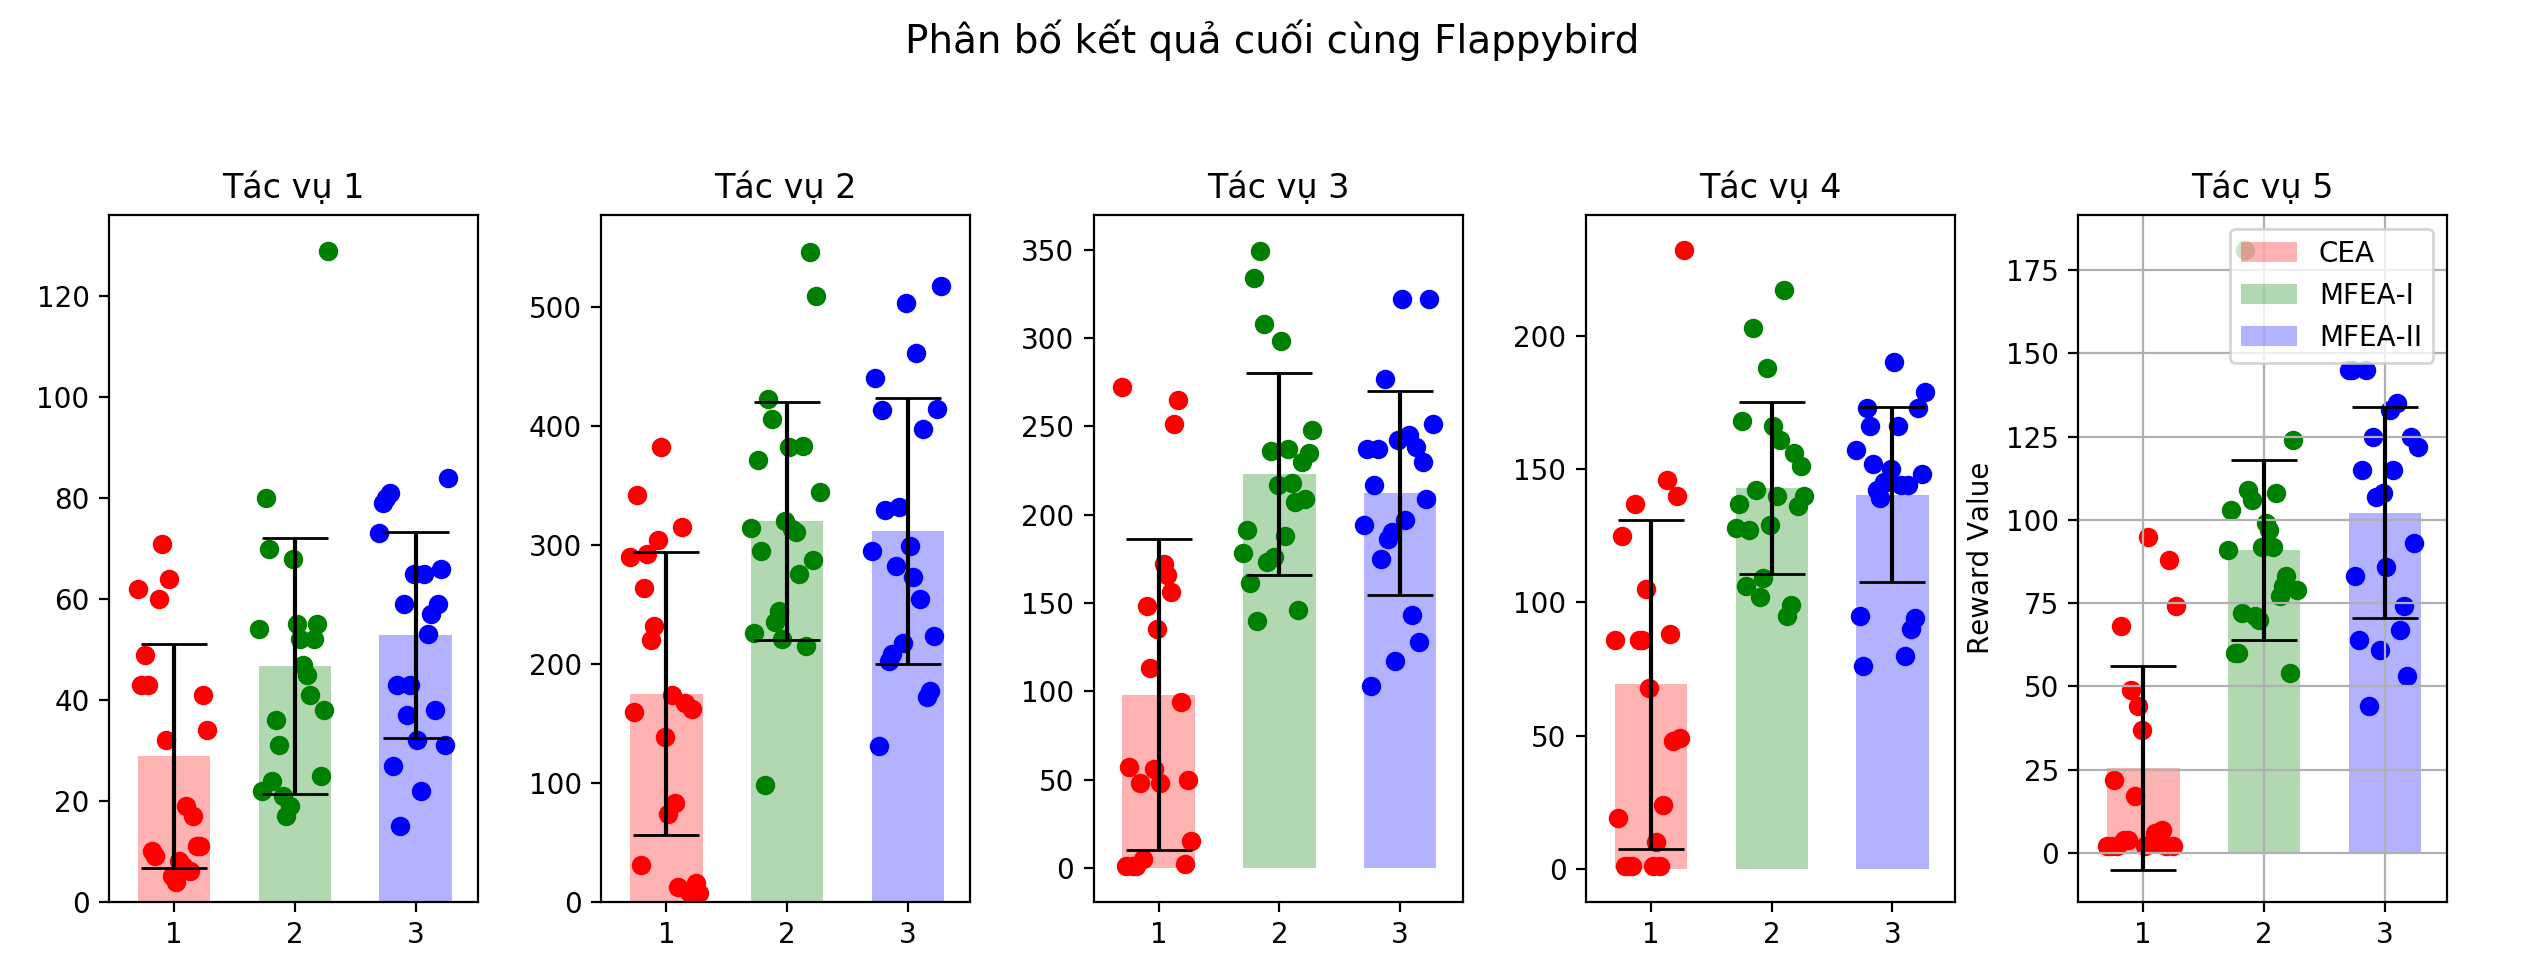
\includegraphics[width=\textwidth,height=\textheight,keepaspectratio]{images/flappybird.png}
        \caption{Flappy Bird}
        \label{fig:FLP}
    \end{figure}
    \end{frame}
    
    \begin{frame}{So sánh biểu độ hội tụ kết quả}
        \begin{figure}[h!]
        \centering
        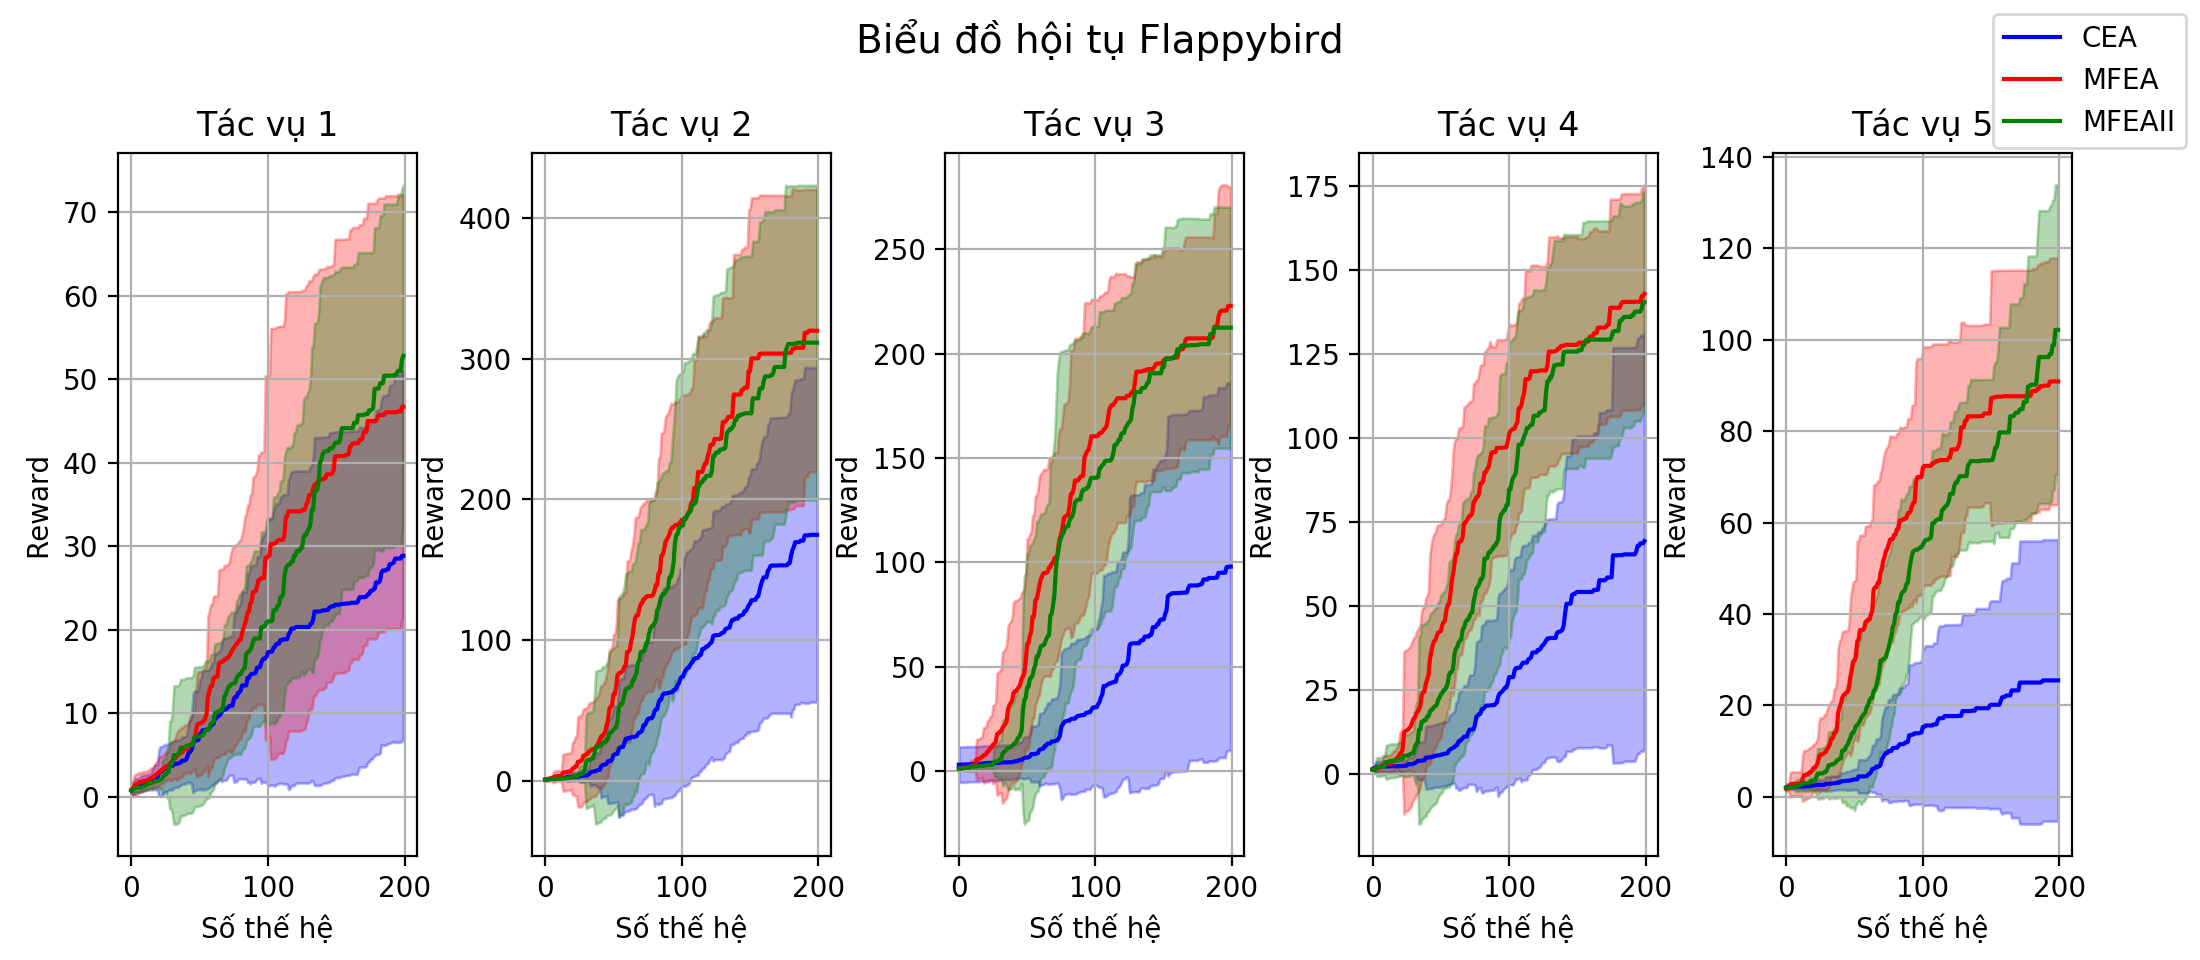
\includegraphics[width=\textwidth,height=\textheight,keepaspectratio]{images/flappybird_conv.png}
        \caption{Flappy Bird}
        \label{fig:FLP}
    \end{figure}
    \end{frame}
    \begin{frame}{So sánh biểu độ hội tụ kết quả Acrobot}
        \begin{figure}[h!]
        \centering
        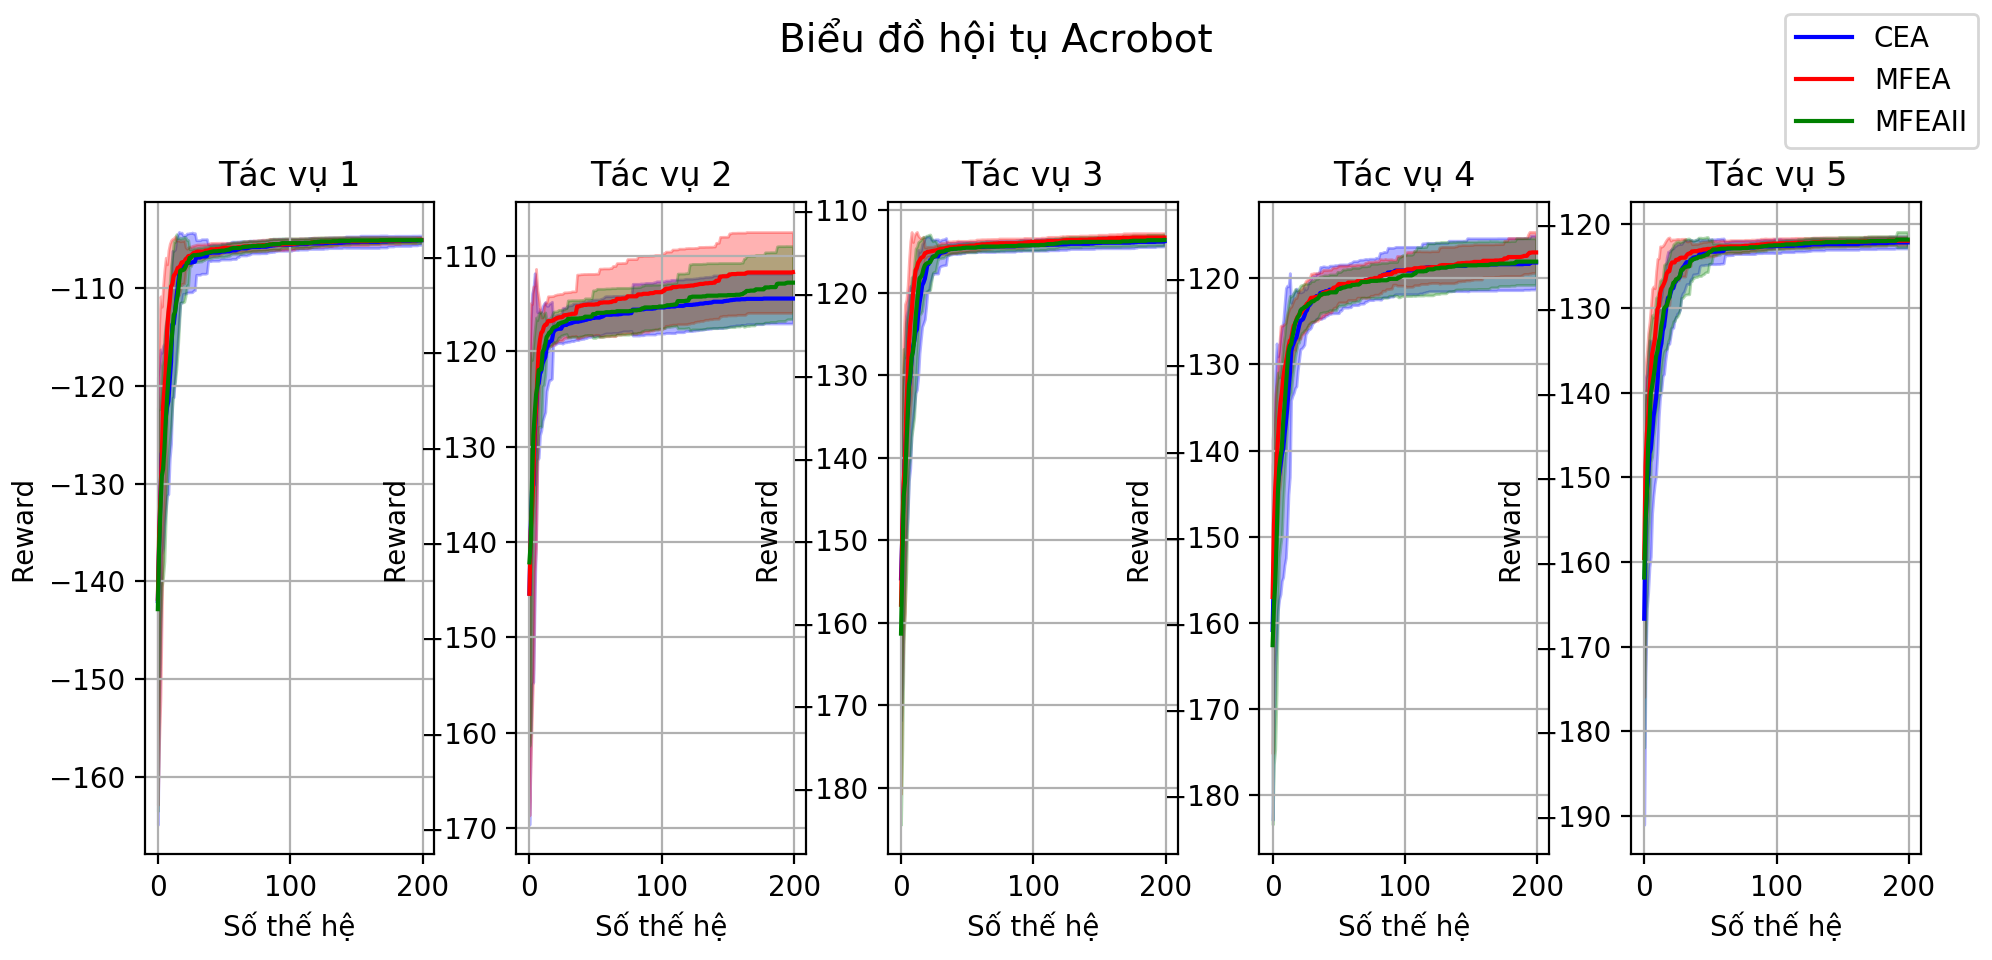
\includegraphics[width=\textwidth,height=\textheight,keepaspectratio]{images/acobot_conv.png}
        \caption{Acrobot}
        \label{fig:Acrobot}
    \end{figure}
    \end{frame}